\documentclass[a4paper, 12pt]{article}
\usepackage[utf8]{inputenc}
\usepackage[english]{babel}
\usepackage[T1]{fontenc}
\usepackage[hidelinks]{hyperref}
\usepackage{commath}
\usepackage{mathtools}
\usepackage{amssymb}
\usepackage{mathrsfs}
\usepackage{libertine}
\usepackage{mortenmath}
\usepackage{graphicx}
\usepackage{cite}
\usepackage{amsmath}
\usepackage{color}
\usepackage{csquotes}
\graphicspath{{Figures/}{./Figures/}}
\usepackage[refpage]{nomencl} \makenomenclature
\usepackage{glossaries}%!TEX root = ../TTK4550-MHT.tex

\nomenclature{$i$}{Measurement index}
\nomenclature{$m_k$}{Number of measurements in scan k}
\nomenclature{$t$}{Time}
\nomenclature{$k$}{Time index}
\nomenclature{$j$}{Target index}
\nomenclature{$t_k$}{Time at time index}
\nomenclature{$l$}{Hypothesis index}
\nomenclature{$\V{x}$}{State vector}
\nomenclature{$\bar{\V{x}}$}{Predicted state}
\nomenclature{$\hat{\V{x}}$}{Filtered state}
\nomenclature{$\M{P}$}{State covariance}
\nomenclature{$\M{\bar{P}}$}{Predicted state covariance}
\nomenclature{$\M{\hat{P}}$}{Filtered state covariance}
\nomenclature{$\V{z}_k$}{Measurement at time step $k$}
\nomenclature{$\M{H}$}{State observation matrix}
\nomenclature{$\M{Q}$}{State covariance matrix}
\nomenclature{$\M{R}$}{Measurement covariance matrix}
\nomenclature{$\M{S}$}{Residual covariance}
\nomenclature{$\M{K}$}{Kalman gain}
\nomenclature{$\V{\nu}$}{Weighted measurement innovation}
\nomenclature{$\mathrm{NLLR}_{i,j}(k)$}{Negative Log Likelihood Ratio for target $j$ at time $k$ for measurement $i$}
\nomenclature{$\mathrm{cNLLR}$}{Cumulative Negative Log Likelihood Ratio for target}
\nomenclature{$\V{\tau}$}{Binary vector where the selected track hypotheses are $1$}
\nomenclature{$\M{\Gamma}$}{Disturbance matrix}
\nomenclature{$\M{\Phi}$}{State transition matrix}
\nomenclature{$\V{w}$}{Process noise}
\nomenclature{$\V{v}$}{Observation noise}
\nomenclature{$N$}{Number of scans to keep in track tree}
\nomenclature{$M$}{Number of leaf nodes (\glspl{track hypothesis} in the \gls{track forest})}
\nomenclature{$N_1$}{Number of real measurements in \gls{cluster}}
\nomenclature{$N_2$}{Number of targets in \gls{cluster}}


%\nomenclature{}{}

%\newglossary[alg]{acronym}{acr}{acn}{Acronyms}
%\newglossaryentry{apc}{name={APC},description={antigeen-presenterende cel}}
%\newglossaryentry{alg:c1}{type=acronym,name={Entry1},description={Desc1}}
%\newglossaryentry{alg:c2}{type=acronym,name={Entry2},description={Desc2}}0
%\newglossaryentry{alg:c3}{type=acronym,name={Entry3},description={Desc3}}
%\makeglossaries

\begin{document}
	\pagenumbering{roman}
	%!TEX root = ../TTK4550-MHT.tex
\begin{titlepage}
\begin{center}
 {\huge\bfseries An ILP approach to \\ Multi Hypothesis Tracking\\}
 % ----------------------------------------------------------------
 \vspace{1.5cm}
 {\Large\bfseries Erik Liland}\\[5pt]
 %erik.liland@gmail.com\\[14pt]
  % ----------------------------------------------------------------
\vspace{2cm} 
{Report  submitted to} \\[5pt]
\emph{{Norwegian University of Science and Technology}}\\[2cm]

% {By}\\[5pt] {\Large \sc {Me}}
 \vfill
 % ----------------------------------------------------------------
{Department of Engineering Cybernetics}\\[5pt]
{O.S. Bragstads Plass 2D}\\[5pt]
{Elektroblokk D, Gløshaugen,\\
7034 Trondheim, Norway}\\
\vfill
{December 2016}
\vfill

\includegraphics[width=0.7\textwidth]{ntnu_logo}\\[5pt]
\end{center}
\end{titlepage}
\clearpage
\newpage

	\addtocounter{page}{1}
	%!TEX root = ../TTK4550-MHT.tex
%ABSTRACT

\begin{abstract}
\addcontentsline{toc}{subsection}{Abstract}
%\vspace*{\fill}
\begin{center}
\emph{\color{red} Tentativ som bare det}

Autonomous surface vessels are, at least in navigational sense, unmanned ships which can be used to transport cargo and people as well as being used for surveillance and other tasks. To ensure a safe journey, the route planer must have a real time image of its surroundings in addition to map data. In the maritime environment, this is primarily done by rotating radars mounted on the ship itself. The challenge then is to know which measurement (reflection) belongs together from scan to scan.
This report documents a survey of multi target tracking methods with a walk-through of derivations and implementations of an N-scan target oriented multi hypothesis tracker algorithm. The algorithm is able to account for missed targets and false measurements. As each set of measurements (scan) is received, the algorithm predicts the position to its known targets and accepts all measurements inside a certain area around the estimated position. Each of the new measurements are scored based on their distance from the estimated position, the uncertainty of the estimate and the (estimated) amount of clutter in each scan. This method allows for correlation of measurements multiple steps back in time, hence average out white noise. The algorithm was tested and found successful on both simulated data with noise as well as recorded data from a S-band maritime radar.
\end{center}
%\vfill
\end{abstract}
\newpage

	\tableofcontents \newpage

	\listoffigures
	\addcontentsline{toc}{section}{List of Figures} \newpage

	\printnomenclature
	\addcontentsline{toc}{section}{Nomenclature} \newpage
	
	%\printglossaries
	%\addcontentsline{toc}{section}{Acronyms} \newpage

	\pagenumbering{arabic}	
	%!TEX root = ../TTK4550-MHT.tex
\section{Introduction}
The aim of this section is to give the reader a feeling for the most popular methods, their assumptions and strong and weak properties as seen from an 2D maritime anti collision perspective.

\subsection{Tracking}
Tracking of an object object (target) is the process of estimating its state (i.e. position and velocity) based on discrete measurements from an observation system. An observation system can be a radar, sonar or any other sensor that passively or actively detects objects within a area or volume. 

\subsection{Tracking system}
A tracking system can be interpreted as either the complete system from the signal processing level to the finished tracks, or as I will I this text: A system that associates consecutive measurements from an observation system, and initiate or assigns them to tracks. A track is a subset of all the measurements from the observation system that is believed to originate from the same target. The challenge with knowing which measurement originating from which (real) target is the core at any tracking system. This association problem is non-trivial even under ideal situations, and the addition of spurious measurements and missed targets only increases the complexity.

There has been developed a large variety of methods to overcome this association problem, and most of them have several sub-methods. In the following subsections, some of the most common and popular methods will be presented.

\subsection{Definitions}
Scan $\triangleq$ a procedure which measures the entire area of coverage of the system. \newline
Measurement $\triangleq$ a point in the measurement space where something is detected.\newline
Score $\triangleq$ a measure of the goodness of a measurement-to-track association. \newline
Dummy measurement $\triangleq$ a self created measurement at the estimated position (with score 0).\newline
Measurement list $\triangleq$ a set of measurement who originate from the same scan. \newline
Target $\triangleq$ an actual object who the system is trying to track. \newline
Track $\triangleq$ a list of measurement indices, one from each scan, who is believed to originate from the same target. \newline
Gate $\triangleq$ an area in which a track expects and approves new measurement to associate with itself. \newline
Track hypothesis $\triangleq$ a new measurement who is inside the gate for an existing track.


\subsection{Nearest Neighbour Standard Filter}
The Nearest Neighbour Standard Filter (NNSF)is the simplest approach in tracking where one always select the closes neighbour as the consecutive measurement in the track. This approach suffers from being very vulnerable from clutter and dense target scenarios, and can be somewhat improved by estimating an a-priori state through a Kalman Filter and selecting the nearest neighbour to the estimate. Even with this extension, it is a very primitive approach which does not yield good real world performance. %Need citeations / corrections

\subsection{Probabilistic Data Association Filter}
Probabilistic Data Association Filter (PDAF) is a \emph{single target} Bayesian association filter which is based on single scan probabilistic analysis of measurements. At each scan the filter is calculating a most probable measurement based on a weighted sum on the measurement innovations inside a validation region.
\begin{equation}
\V{\hat{y}} \triangleq \sum\limits_{j=1}^m \beta_j \V{ \tilde{y}_j }
\label{PDA_sum}
\end{equation}
where $\beta_j$ is the probability of measurement j to be the correct one, and $ \tilde{y}_j = y_j - \hat{y}_j $ is the j-th measurement innovation. 

PDAF is computationally modest (approximate 50\% more computationally demanding than a Kalman Filter \cite{Bar-Shalom1988} p.163) and have good results in an environment with up to about 5 false measurement in a $4\sigma$ validation region \cite{Bar-Shalom1988}. PDAF does not include track initialisation and assumes that at most one measurement can originate from an actual target. It also assumes that clutter is uniformly distributed in the measurement space and that the targets history is approximated by a Gaussian with a calculated mean and covariance (single scan).

PDAF can be used for multiple targets, but only as multiple copies of the single-target filter \cite{Fortmann1983}. Since PDAF is generating a "best guess"-measurement from all the measurements inside its validation region, it can suffer from track coalescence. This coalescence occurs when two targets have similar paths, and the resulting tracks will be an "average" of the two (actual) tracks.
PDAF is considered the simplest "state of the art" tracking algorithm.%Needs citation / correction


\subsection{Joint Probabilistic Data Association Filter}
Joint Probabilistic Data Association Filter (JPDAF) is a \emph{multi target} extension of the Probabilistic Data Association Filter in which joint posteriori association probabilities are calculated for every target at each scan. Both PDAF and JPDAF use the same weighted sum (\ref{PDA_sum}), the key difference is the way the weight $ \beta_j $ is calculated. Whereas PDAF treats all but one measurement inside its validation region as clutter, in JPDAF the targets who interacts (one cluster) are treated as connected and the connected $ \beta_j $s are computed jointly across the cluster set with a given set of active targets inside the cluster. The probability of a measurement $j$ belonging to a target
$ t $ is \cite{Fortmann1983}
\begin{equation}
\begin{split}
\beta_j^t &= \sum_{\chi} P\{ \chi | Y^k \} \hat{\omega}_{jt}(\chi) \\
\beta_0^t &= 1 - \sum_{j=1}^m \beta_j^t
\end{split}
\end{equation}
where
\begin{equation}
P\{\chi|Y^k\} = \frac{C^\phi}{c} 
				\prod_{j:\tau_j=1} \frac{exp[-\frac{1}{2}(\V{\tilde{y}_j^{t_j}})^T S_{t_j}^{-1}(\V{\tilde{y}^{t_j}})]}{(2\pi)^{M/2} |S_{t_j}|^{1/2}}
				\prod_{t:\delta_t=1} P_D^t
				\prod_{t:\delta_t=0} (1 - P_D^t)
\end{equation}

Since the JPDAF is calculating joint probability for all the combinations of measurement associations in the cluster, the computation demand is growing exponentially with the numbers of tracks and measurements in the cluster. A real time implementation of the JPDAF has been developed and patented by QinetiQ \cite{QinetiQ2003}, and an approach for avoiding track coalescence has been proposed by \cite{Blom2000}.                                                   

\subsection{Multi Hypothesis Tracker}
Multiple hypothesis tracking (MHT) is a category of methods that are based around the concept of evaluating multiple  combinations of measurements to data association, and rank them with respect to their statistical properties. In contrast to PDA methods which in some cases will estimate an "average" of two tracks as the true on (coalesce), MHT methods split when in doubt. The original MHT algorithm was presented in \cite{Reid1978}, where a hypothesis oriented MHT was developed. Following this, a track oriented MHT was proposed in \cite{Kurien1990} and improved by \cite{Bar-Shalom2007}.

\subsubsection{Hypothesis Oriented MHT}
Hypothesis Oriented Multiple Hypothesis Tracker (HOMHT) or Measurement Oriented Multiple Hypothesis Tracker (MOMHT) is on a fully Bayesian approach where direct probabilities of global joint measurement to target association hypothesis are calculated. The algorithm initiates track and handles missing measurements, has a recursive nature and is allows for clustering for quicker calculations. One of the main benefits of MHT is the ability to utilize multiple scans to aid in the data association, in other words to use all the available data when taking decisions. TOMHT was developed under the assumption that no target can originate more than one measurement from each scan, and a target does not necessary show on every scan. When evaluating the probability of a hypothesis, the MHT takes into account the false-alarm statistics of the measurement system, the expected density of targets and clutter and the accuracy of the target estimates.

The probability of each data association hypothesis was developed by Reid in \cite{Reid1978}
\begin{equation}
P_i^k = \frac{1}{c} P_D^{N_{DT}}(1-P_D)^{(N_{TGT}-N_{DT})} \beta_{FT}^{N_{FT}} \beta_{NT}^{N_{NT}} \left[ \prod_{m=1}^{N_{DT}} N(\V{Z_m}-\M{H}\V{\bar{x}},\M{B}) \right] P_g^{k-1}
\end{equation}
where $P_i^k$ is the probability of hypothesis $\Omega_i^k$ given measurements up through time $k$. $P_D$ is the probability of detection, $\beta_{FT}$ is the density of targets, $\beta_{NT}$ is the density of previously unknown targets that have been detected, $N_{DT}$ is number of designated targets, $N_{FT}$ is the number of false targets, $N_{NT}$ is the number of new targets, $N_{TGT}$ is the number of targets, $\V{Z_m}$ is the m-th measurement in the current scan, $\M{H}$ is the observation matrix and $\M{B}$ is the measurement covariance.

\subsubsection{Track Oriented MHT}
Track Oriented Multiple Hypothesis Tracker (TOMHT) is a "bottom-up" approach where the tracks are assumed initialized, and for each scan the track split whenever there are more than one feasible measurement in the validation region. The new track hypothesis state is generated from the posteriori filtered estimate from a Kalman Filter, and a score/cost is calculated using (20) from \cite{Bar-Shalom2007}. Following the addition of a new track hypothesis, the tracks are divided into clusters where all tracks who share measurements from the latest scan are in one cluster. The clusters must then be analysed to find the beast possible combination of mutual exlucsivemeasurement associations. LP- and ILP-based methods as proposed by \cite{Storms2003} can be used to find the best (nearest optimal) combinations of newly created track hypothesis in accordance to the assumption that a measurement only can be assigned to one target and that one target can maximally create one measurement.

To limit the size of the track hypothesis tree some sort of pruning/elimination of unlikely hypothesis must be carried out. ""This step is, from a Bayesian point of view, the most problematic since ...""




	
%!TEX root = ../TTK4550-MHT.tex
\section{Survey of multi-target tracking methods}
\label{sec:survey}
The aim of this section is to give the reader a brief overview of tracking as a problem and a feeling for the most popular methods, their assumptions and strong and weak properties as seen from an 2D maritime anti collision perspective.

\subsection{Tracking}
Tracking of an object (target) is the process of estimating its state (i.e. position and velocity) based on discrete measurements from an observation system. An observation system can be a radar, sonar or any other sensor that passively or actively detects objects within an area or volume.

\subsection{Tracking system}
A tracking system can be interpreted as either the complete system from the signal processing level to the finished tracks, or as in this text: \emph{A system that associates consecutive measurements from an observation system, and initiate or assigns them to tracks.} A track is a subset of all the measurements from the observation system that is believed to originate from the same target. The challenge knowing which measurement originating from which (real) target is the core at any tracking system. This association problem is non-trivial even under ideal situations, and the addition of spurious measurements and missed targets only increases the complexity.

There has been developed a large variety of methods to overcome this association problem, and most of them have several sub-methods. In the following subsections, some of the most common and popular methods will be presented.

\subsection{Nearest Neighbor Filter}
The Nearest Neighbor Filter (NNF)is the simplest approach in tracking, where one always select the closes neighbor as the consecutive measurement in the track. This approach suffers from being very vulnerable to clutter and dense target scenarios. It can be somewhat improved by estimating an a-priori state through a Kalman Filter and selecting the nearest neighbor to the estimate. This extension is sometimes refereed to as Nearest Neighbor Standard Filter (NNSF). Under the (normal) assumption that each target can at maximum generate one measurement, the NNF and NNSF are both single-target methods. They can however be expanded to multi-target variants by formulating the problem as a global least squares integer optimization problem. With this extension the NNSF is almost becoming a zero-scan multi hypothesis tracker. NNF and NNSF are the only method presented which is non-probabilistic, and does not assume specific models for noise, etc.

\subsection{Probabilistic Data Association Filter}
Probabilistic Data Association Filter (PDAF) is a \emph{single-target} Bayesian association filter which is based on single scan probabilistic analysis of measurements. At each scan the filter is calculating a most probable measurement based on a weighted sum on the measurement innovations inside a validation region.
\begin{equation}
\V{\hat{y}} \triangleq \sum\limits_{j=1}^m \beta_j \V{ \tilde{y}_j }
\label{PDA_sum}
\end{equation}
where
\begin{equation*}
\begin{split}
	\beta_j		&= \text{the probability of measurement j to be the correct one} \\
	\tilde{y}_j &= y_j - \hat{y}_j \hspace{5mm}	\text{the j-th measurement innovation}
\end{split}
\end{equation*}
PDAF is computationally modest (approximate 50\% more computationally demanding than a Kalman Filter \cite{Bar-Shalom1998} p.163) and have good results in an environment with up to about 5 false measurement in a $4\sigma$ validation region \cite{Bar-Shalom1998}. PDAF does not include track initialization and assumes that at most one measurement can originate from an actual target. It also assumes that clutter is uniformly distributed in the measurement space and that the targets history is approximated by a Gaussian with a calculated mean and covariance (single scan).

PDAF can be used for multiple targets, but only as multiple copies of the single-target filter \cite{Fortmann1983}. Since PDAF is generating a "best guess"-measurement from all the measurements inside its validation region, it can suffer from track coalescence. This coalescence occurs when two targets have similar paths, and the resulting tracks will be an "average" of the two (actual) tracks. There has been done some work to overcome this coalescence \cite{Blom2000}.


\subsection{Joint Probabilistic Data Association Filter}
Joint Probabilistic Data Association Filter (JPDAF) is a \emph{multi-target} extension of the Probabilistic Data Association Filter in which joint posteriori association probabilities are calculated for every target at each scan. Both PDAF and JPDAF use the same weighted sum (\ref{PDA_sum}), the key difference is the way the weight $ \beta_j $ is calculated. Whereas PDAF treats all but one measurement inside its validation region as clutter, in JPDAF the targets which interacts (one cluster) are treated as connected and the connected $ \beta_j $s are computed jointly across the cluster set with a given set of active targets inside the cluster. The probability of a measurement $j$ belonging to a target
$ t $ is \cite{Fortmann1983}
\begin{equation}
\begin{split}
\beta_j^t &= \sum_{\chi} P\{ \chi | Y^k \} \hat{\omega}_{jt}(\chi) \\
\beta_0^t &= 1 - \sum_{j=1}^m \beta_j^t
\end{split}
\end{equation}
where
\begin{equation}
P\{\chi|Y^k\} = \frac{C^\phi}{c} 
				\prod_{j:\tau_j=1} \frac{exp[-\frac{1}{2}(\V{\tilde{y}_j^{t_j}})^T S_{t_j}^{-1}(\V{\tilde{y}^{t_j}})]}{(2\pi)^{M/2} |S_{t_j}|^{1/2}}
				\prod_{t:\delta_t=1} P_D^t
				\prod_{t:\delta_t=0} (1 - P_D^t).
\end{equation}
Where 
\begin{equation*}
\begin{split}
	\beta_j^k			&= \text{the probability that measurement j belongs to target k} \\
	\beta_0^k 			&= \text{the probability that no measurement belongs to target k} \\
	\chi 				&= \text{All feasible events} \\
	Y^k 				&= \text{all candidate measurements up to and included time k} \\
	\hat{\omega}_{jt}	&=	\begin{cases}
								1, \text{if } \chi_{jt} \text{ occurs} \\ 
								0, \text{otherwise} 
							\end{cases} \\
	m					&= \text{number of measurements}
\end{split}
\end{equation*}
Since the JPDAF is calculating joint probability for all the combinations of measurement associations in the cluster, the computation demand is growing exponentially with the numbers of tracks and measurements in the cluster. A real time implementation of the JPDAF has been developed and patented by QinetiQ \cite{QinetiQ2003}, and described in \cite{Horridge}, and an approach for avoiding track coalescence has been proposed by \cite{Blom2000}.

\subsection{Multi Hypothesis Tracker}
Multiple hypothesis tracking (MHT) is a category of methods that are based around the concept of evaluating multiple combinations of measurements to data association, and rank them with respect to their score. In contrast to PDA methods which in some cases will estimate an "average" of two tracks as the true on (coalesce), MHT methods split when in doubt. The original MHT algorithm was presented in \cite{Reid1978}, where a hypothesis oriented MHT was developed. Following this, a track oriented MHT was proposed in \cite{Kurien1990} and improved by \cite{Bar-Shalom2007}.

\subsubsection{Hypothesis Oriented MHT}
Hypothesis Oriented Multiple Hypothesis Tracker (HOMHT) or Measurement Oriented Multiple Hypothesis Tracker (MOMHT) is a fully Bayesian approach where direct probabilities of global joint measurement-to-target association hypothesis are calculated. The algorithm initiates tracks and handles missing measurements, it has a recursive nature and it allows for clustering for quicker computation. One of the main benefits of MHT is the ability to utilize multiple scans (history) to aid in the data association, in other words to use all the available data when taking decisions. TOMHT was developed under the assumption that at most one measurement can originate from each target in each scan, and that a target does not necessary show on every scan (Probability of detection, $P_D < 1$). When evaluating the probability of a hypothesis, the MHT takes into account the false-alarm statistics of the measurement system, the expected density of targets and clutter and the accuracy of the target estimates.

The probability of each data association hypothesis was developed by Reid in \cite{Reid1978}
\begin{equation}
P_i^k = \frac{1}{c} P_D^{N_{DT}}(1-P_D)^{(N_{TGT}-N_{DT})} \beta_{FT}^{N_{FT}} \beta_{NT}^{N_{NT}} \left[ \prod_{m=1}^{N_{DT}} N(\V{Z_m}-\M{H}\V{\bar{x}},\M{B}) \right] P_g^{k-1}
\end{equation}
where 
\begin{equation*}
\begin{split}
	P_i^k		&= \text{the probability of hypothesis $\Omega_i^k$ given measurements up through time $k$} \\
	P_D 		&= \text{the probability of detection} \\
	\beta_{FT} 	&= \text{the density of targets} \\
	\beta_{NT}	&= \text{the density of previously unknown targets that have been detected} \\
	N_{DT} 		&=	\text{number of designated target} \\
	N_{FT} 		&= \text{the number of false targets} \\
	N_{NT} 		&= \text{the number of new targets} \\
	N_{TGT} 	&= \text{is the number of targets} \\
	\V{Z_m} 	&= \text{the m-th measurement in the current scan} \\
	\M{H} 		&= \text{the observation matrix} \\
	\M{B} 		&= \text{the measurement covariance}
\end{split}
\end{equation*}

\subsubsection{Track Oriented MHT}
Track Oriented Multiple Hypothesis Tracker (TOMHT) is a "bottom-up" approach where the tracks are assumed initialized, and for each scan the track splits whenever there are more than one feasible measurement in the validation region (in addition to the no-measurement hypothesis). The new track hypothesis state is generated from the posteriori filtered estimate from a Kalman Filter, and a score/cost is calculated using (20) from \cite{Bar-Shalom2007}. Following the addition of a new track hypothesis, the tracks are divided into clusters where all tracks which share measurements from the N-latest scan are in one cluster. The clusters can then be analyzed as standalone global problems to find the beast possible combination of (possibly mutual exclusive) measurement associations. Linear programming (LP)- and Integer Linear Programming (ILP)-based methods as proposed by \cite{Storms2003} can be used to find the best combinations of newly created track hypotheses in accordance to the assumption that a measurement only can be assigned to one target and that one target can maximally create one measurement.

To limit the size of the track hypothesis tree, the unused edges of the track hypothesis tree will be removed after N scans.

 
	%!TEX root = ../TTK4550-MHT.tex
\section{Algorithm walk-through}
\label{sec:algorithm}
\subsection{Flowchart}
Figure \ref{fig:algorithm_flow} shows a flowchart of the track oriented MHT algorithm presented in this section. An important difference between this approach compared to Reid's original measurement oriented MHT \cite{Reid1978}, is the need for external initialization of targets.
\begin{figure}[ht]
\centering
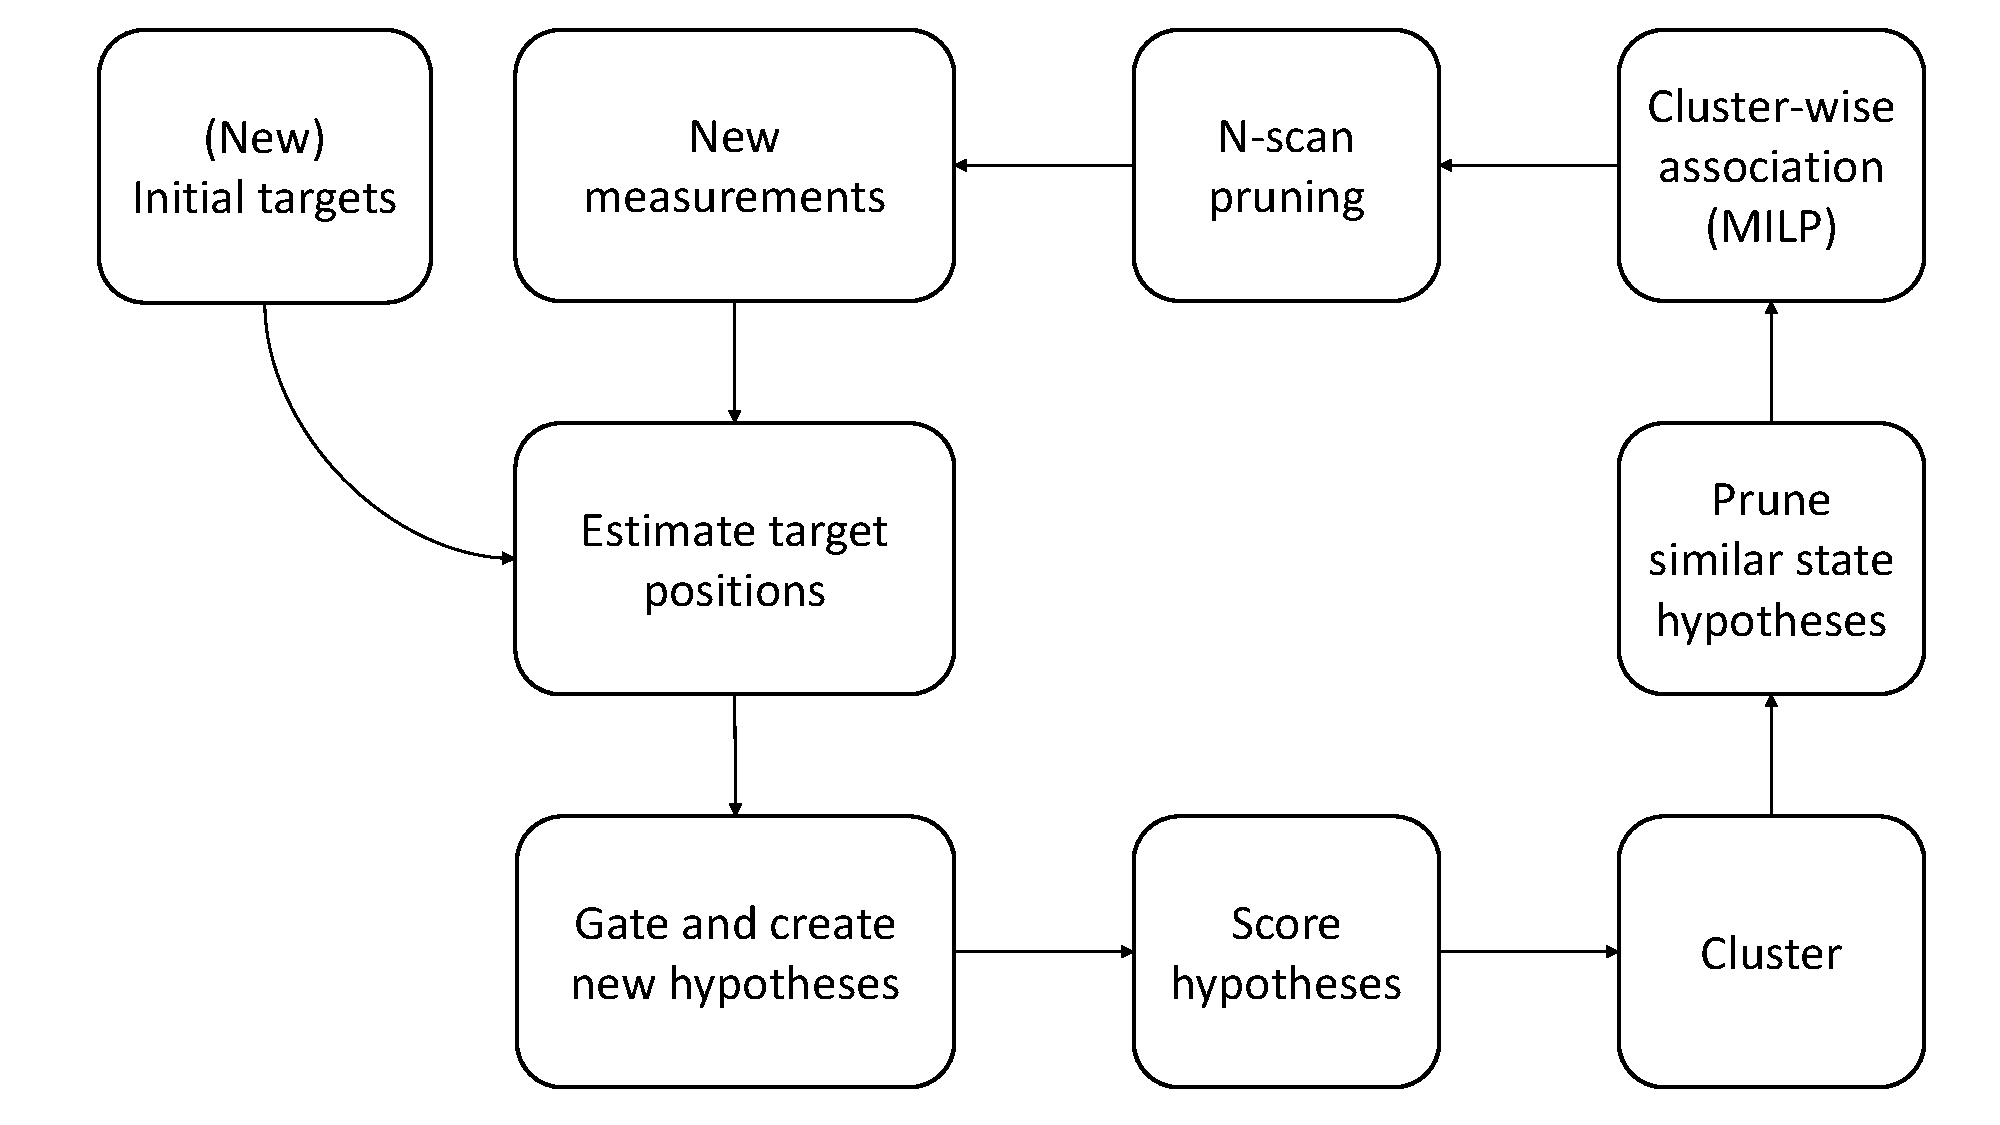
\includegraphics[width = .9\textwidth]{algorithm_flowchart.pdf}
\caption{Algorithm flowchart}
\label{fig:algorithm_flow}
\end{figure}

\subsection{State estimation}
When a new set of measurement is arriving, it is desirable to "guess" where the target might be before looking for matching measurements. This can be done though a model of the targets dynamics and a state estimator. For the purpose of tracking ships in a local frame (Cartesian plane), we compose a state vector with four states
\begin{equation}
\V{x} = \begin{bmatrix}
x & y & \dot{x} & \dot{y}
\end{bmatrix}^T
\label{eq:state_vector}
\end{equation}
where the change of velocity (acceleration) is assumed zero. The latest assumption is compensated with an increased system noise covariance in the model. For a linear system, a Kalman Filter is an optimal estimator which have the following time evolution assumptions.
\begin{equation}
\begin{split}
\V{x}(k+1) &= \M{\Phi} \V{x}(k) + \M{\Gamma} \V{w} \\
\V{z}(k) &= \M{H} \V{x}(k) + \V{v}
\end{split}
\label{eq:kalman_timeUpdate}
\end{equation}
where
\begin{equation}
\begin{split}
\M{\Phi} 	&= \text{the state transition matrix} \\
\M{\Gamma}	&= \text{the disturbance matrix} \\
\V{w}		&= \text{the process noise} \\
\M{H} 		&= \text{the measurement matrix} \\
\V{v} 		&= \text{the observation noise} \\
\end{split}
\end{equation}.
The procedure of estimating the target state at the next time step is according to the "time update" equations of the Kalman Filter.
\begin{equation}
\begin{split}
\V{\bar{x}}(k+1) 	&= \M{\Phi} \V{\hat{x}}(k) \\
\M{\bar{P}}(k+1)	&= \M{\Phi} \M{\hat{P}}(k)  \M{\Phi}^T + \M{Q} \\
\end{split}
\end{equation}
Where Q is the system covariance matrix. The model have the following parameters,
\begin{equation*}
\M{\Phi} =	\begin{bmatrix}
1 & 0 & T & 0 \\
0 & 1 & 0 & T \\
0 & 0 & 1 & 0 \\
0 & 0 & 0 & 1 \\
\end{bmatrix} \quad
\M{\Gamma} = \begin{bmatrix}
0 & 0 \\
0 & 0 \\
1 & 0 \\
0 & 1 \\
\end{bmatrix} \quad
\M{H} = \begin{bmatrix}
1 & 0 & 0 & 0 \\
0 & 1 & 0 & 0 \\
\end{bmatrix}
\end{equation*}
\begin{equation*}
\M{Q}	= \sigma_v^2 \begin{bmatrix}
\frac{T^3}{3} 	& 0 				& \frac{T^2}{2}	& 0 			\\
0 				& \frac{T^3}{3}  	& 0 			& \frac{T^2}{2}	\\
\frac{T^2}{2}	& 0					& T				& 0				\\
0				& \frac{T^2}{2}		& 0				& T				\\
\end{bmatrix} \quad
\M{R} = \sigma_r^2 \begin{bmatrix}
1 & 0 \\
0 & 1 \\
\end{bmatrix}
\end{equation*}
where $T$ is the time between the current and the previous measurement, $\sigma_v^2$ is the system velocity variance and $\sigma_r^2$ is the measurement variance. This model is very common due to its simplicity, and is used in among others \cite{Reid1978}, \cite{Coraluppi2000} and \cite{Brekke2012}.

\subsection{Gating}
To avoid calculating the likelihood for all possible combinations of targets and measurements, some sort of selection criteria is needed when creating new hypotheses. One way of doing this gating is to select all measurements that are within a certain confidence region (generally an ellipsoid), as done in \cite{Reid1978}.

\begin{gather*}
\M{B}	= \M{H} \M{\bar{P}} \M{H}^T + \M{R} \\
(\V{Z_m} - \M{H}\V{\bar{x}})^T	\M{B}^{-1} (\V{Z_m} - \M{H}\V{\bar{x}}) \leq \eta^2
\end{gather*}
Where $\eta$ is the gate size.  Chi-Square value with a given confidence interval and two degrees of freedom. For each measurement inside the region, calculate the a posteriori state and covariance using the "measurement update" equations in the Kalman Filter (\ref{eq:kalman_measurementUpdate}) and create a new hypothesis with this state and covariance as initial.

\begin{table}
\begin{tabular}{c c c c c c c c}
Confidence 	& 70\% 	& 80\% 	& 90\% 	& 95\% 	& 97.5\% 	& 99\% 	& 99.5\% \\ \hline
$\eta^2$ 	& 2.41 	& 3.22 	& 4.61 	& 5.99 	& 7.38 		& 9.21 	& 10.60
\end{tabular}
\caption{$\chi^2$ values for two degrees of freedom for selected confidence values}
\label{tab:chi_square}
\end{table}

\begin{figure}[ht]
\centering
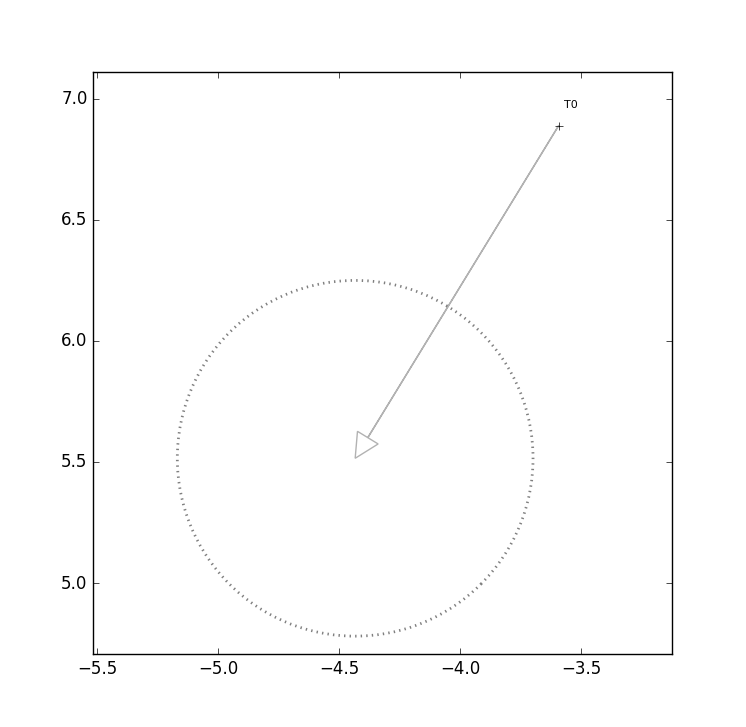
\includegraphics[clip, trim = 1.5cm 1cm 1.5cm 1.5cm,width = .95\textwidth]{ex1-validationRegion}
\caption{Validation region}
\label{fig:validation_region}
\end{figure}

\begin{equation}
\begin{split}
\V{\tilde{y}}	&= \V{z} - \M{H} \V{\bar{x}} \\
\M{S}			&= \M{H} \M{\bar{P}} \M{H}^T + \M{R} \\
\M{K} 			&= \M{\bar{P}} \M{H}^T \M{S}^{-1} \\
\V{\hat{x}}(k) 	&= \V{\bar{x}} + \M{K} \V{\tilde{y}} \\
\M{\hat{P}}(k) 	&= \left( \M{I} - \M{K} \M{H} \right) \M{\bar{P}}
\end{split}
\label{eq:kalman_measurementUpdate}
\end{equation}

\subsection{Scoring}
Each hypothesis are scored according to \cite{Bar-Shalom2007}:
\begin{equation}
\begin{split}
NLLR_{t,j}(k) &= \frac{1}{2} \left[ \tilde{y}_k^T S_{tj}(k)^{-1} \tilde{y}_k \right] + \ln \frac{\lambda_{ex} |2 \pi S_{tj}(k)|^{1/2}}{P_{D_t}(k)} \\				
\tilde{y}_k &= z_j(k)-\hat{z}_t(k|k-1)
\end{split}
\end{equation}
where the cumulative NLLR is
\begin{equation}
l_t^k \triangleq \sum_{l=0}^k NLLR_{t,j(t,l)}(l)
\end{equation}

\subsection{Clustering}
Since the global problem of finding the optimal selection of hypotheses is growing exponentially with the number of hypotheses, it is computationally beneficial to split the problem into smaller problem. This can only be done to targets that does not share any measurements within the N-latest time step. This is done efficiently through breath-first-search or depth-first-search on a graph made from the hypothesis tree.

\subsection{Association}
When the targets are divided into independent clusters, each of them can be treated as a global problem where we want to minimize the cost of the selected hypotheses (leaf nodes), while fulfilling the constraints that each measurement can only be a part of one track and that minimum and maximum one hypothesis can be selected from each target. Since only binary values, selected of not selected, is desired for selection of hypotheses, the problem becomes a integer linear optimization problem.

\subsection{N-scan pruning}
To keep the computational cost within reasonable limits, it is necessary to limit the amount of time steps backwards in time that the algorithm computes. This is done by removing all but the active hypothesis at the current root node, and assign the remaining hypothesis as new root node. 

\begin{figure}[ht]
\centering
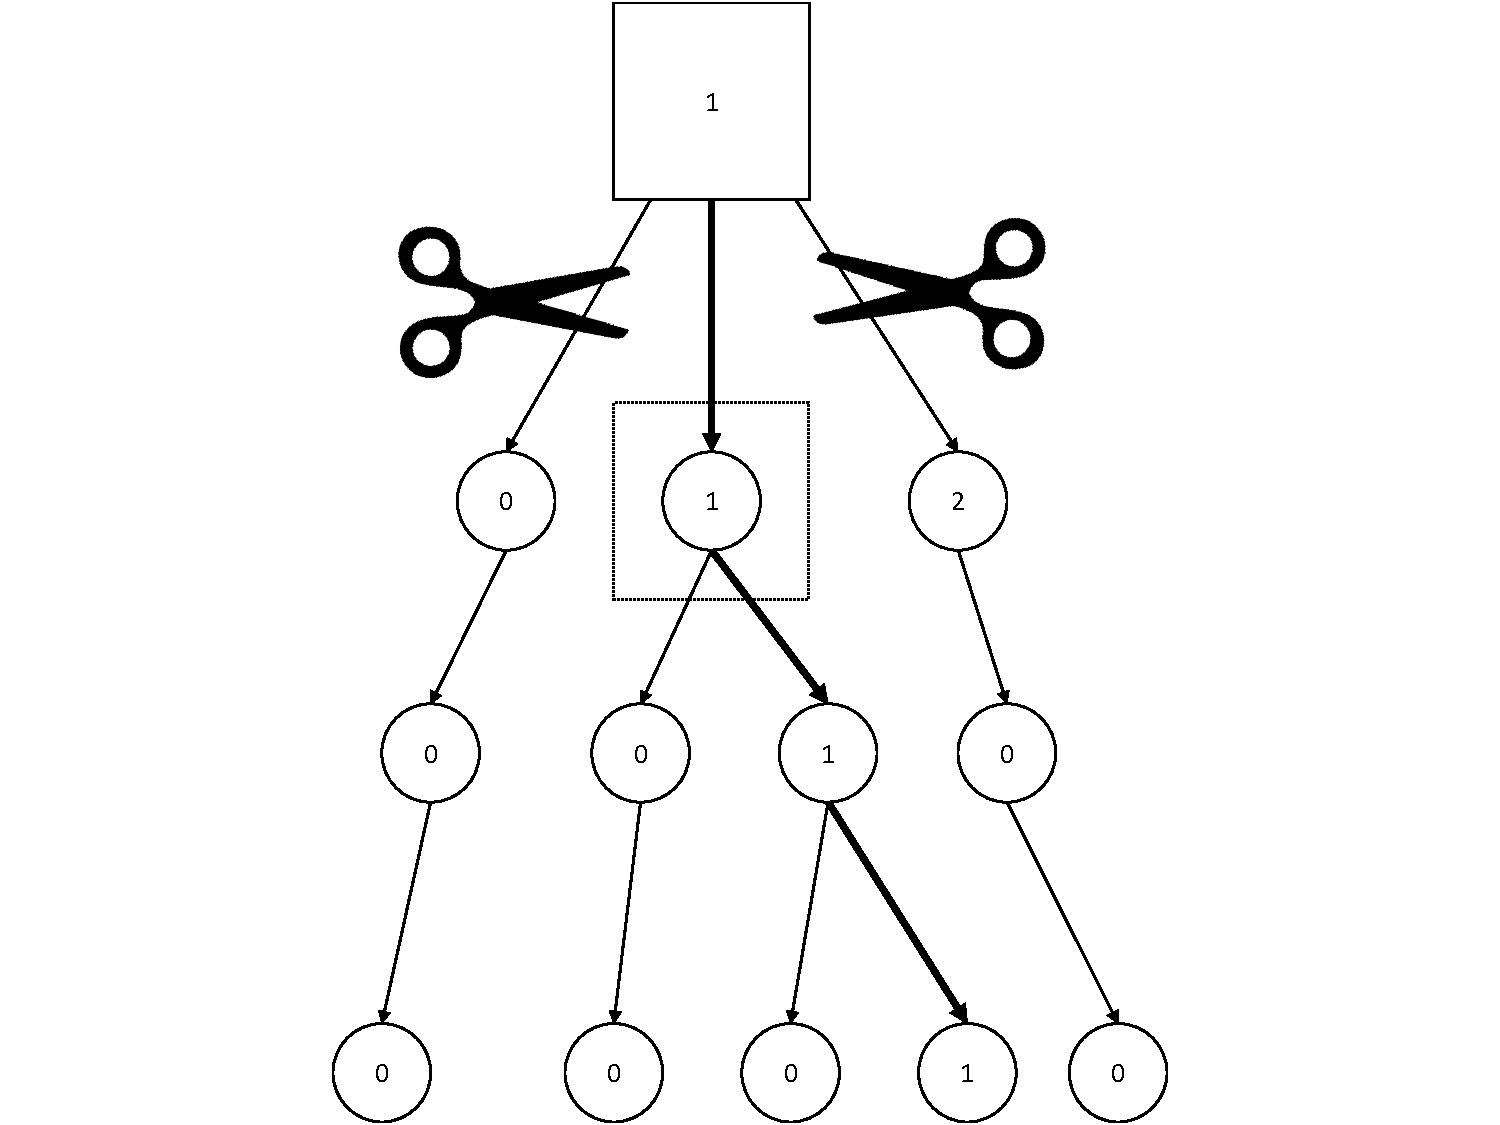
\includegraphics[clip, trim = 2cm 0cm 2cm 0cm,width = .8\textwidth]{Pruned-tree.pdf}
\caption{Pruned track hypothesis tree}
\label{fig:pruned-hyp-tree}
\end{figure}
	%!TEX root = ../TTK4550-MHT.tex
\section{Linear programming}
\label{sec:ilp}
The aim of this section is to elaborate the use of \gls{lp} to solve the data association problem in \gls{mht} that arises when there are multiple (possible mutual exclusive) possibilities of measurement arrangements within the existing set of tracks. As with any optimization problem, we need an objective function which tells us how good or bad a given assignment is, and a set of constraints that limits the solution to physical limits and our assumptions.

\subsection{Problem formulation}
Multiple optimization formulations of the association problem for multi-target tracking have been proposed through the history. The first was \cite{Morefield1977} where a 0-1 \gls{ilp} was proposed, later an \gls{ilp} scheme with \gls{lp} relaxation and \gls{grp} as solver was proposed by \cite{Storms2003}, and a framework for both association and removal of competing tracks were proposed by \cite{Coraluppi2004}.

All three mentioned publications have essentially the same objective functions, though some use minimize and other use maximize in their formulation. The essence of them all is (\ref{eq:general_objective_funtion}), where $\V{c}$ is a vector of costs (minimize) or scores (maximize) and $\V{\tau}$ is a selection vector, where each row in $\V{c}$ and $\V{\tau}$ represents one branch in the track hypothesis tree.
\begin{equation}
\begin{aligned}
& \underset{\V{\tau}}{\text{min}}
& & \V{c}^T \V{\tau}
\end{aligned}
\label{eq:general_objective_funtion}
\end{equation}

Further, the constraints that shall ensure that each measurement is not assigned to more  than one track are generally formulated as (\ref{eq:general_constraints_equality}) or (\ref{eq:general_constraints_inequality}) , where $\M{A}$ is a binary matrix whose rows are branches in a track hypothesis tree and $\V{b}$ is a vector with ones.
\begin{equation}
\begin{aligned}
&	\M{A} \V{\tau} = \V{b} 	\\
&	\V{\tau} \in \{0,1\}^M
\end{aligned}
\label{eq:general_constraints_equality}
\end{equation}

\begin{equation}
\begin{aligned}
&	\M{A} \V{\tau} \leq \V{b} 	\\
&	\V{\tau} \in \{0,1\}^M
\end{aligned}
\label{eq:general_constraints_inequality}
\end{equation}
The difference between (\ref{eq:general_constraints_equality}) and (\ref{eq:general_constraints_inequality}) originates in some fundamental assumptions in different \gls{mht} versions. When used on a \gls{homht} tree, (\ref{eq:general_constraints_equality}) includes track initialization since it demands that all measurements must be assigned. On the other hand, both (\ref{eq:general_constraints_inequality}) and (\ref{eq:my_constraints}) requires a-priori knowledge about the number of tracks.

In this work, the problem is formulated slightly different, in that there are two sets of constraints (\ref{eq:my_constraints}), one equality and one inequality. The inequality constraints $\M{A_1} \V{\tau} \leq \V{b_1}$ ensures that each measurement are maximum (but not minimum) used one time. The equality constraints $\M{A_2} \V{\tau} = \V{b_2}$ ensures that minimum and maximum one track from each track tree is selected. The complete \gls{ilp} formulation becomes (\ref{eq:my_constraints}), where $\V{\tau}$ is a binary vector with dimension equal the number of leaf nodes in the track forest.
\begin{equation}
\begin{aligned}
&	\underset{\V{\tau}}{\text{max}}
&&	\V{c}^T \V{\tau} \\
&	\text{s.t.}
&&	\M{A_1} \V{\tau} \leq \V{b_1} 	\\
&&&	\M{A_2} \V{\tau} = \V{b_2}	\\
&&&	\V{\tau} \in \{0,1\}^M
\end{aligned}
\label{eq:my_constraints}
\end{equation}
$\M{A_1}$ is a $N_1 \times M$ binary matrix with $N_1$ real measurements and $M$ track hypotheses (all leaf nodes), where $\M{A_1}(l,i)=1$ if hypothesis $l$ are utilizing measurement $i$, $0$ otherwise. The measurements and hypothesis are indexed by the order they are visited by \gls{dfs}. $\M{A_2}$ is an $N_2 \times M$ binary matrix where $N_2$ is the number of targets in the cluster and $\M{A_2}(l,j)=1$ if hypothesis $l$ belongs to target $j$. $\V{b_1}$ is a $N_1$ long vector with ones and $\V{b_2}$ is a $N_2$ long vector with ones. $\V{c}$ is a $M$ long vector with a measure of the goodness of the track hypotheses. For example, in Figure \ref{fig:hyp-tree} at time step 2, the $\M{A}$ matrices and $\V{C}$ vector would be (\ref{eq:example_matrices}).
\begin{figure}[H]
\centering
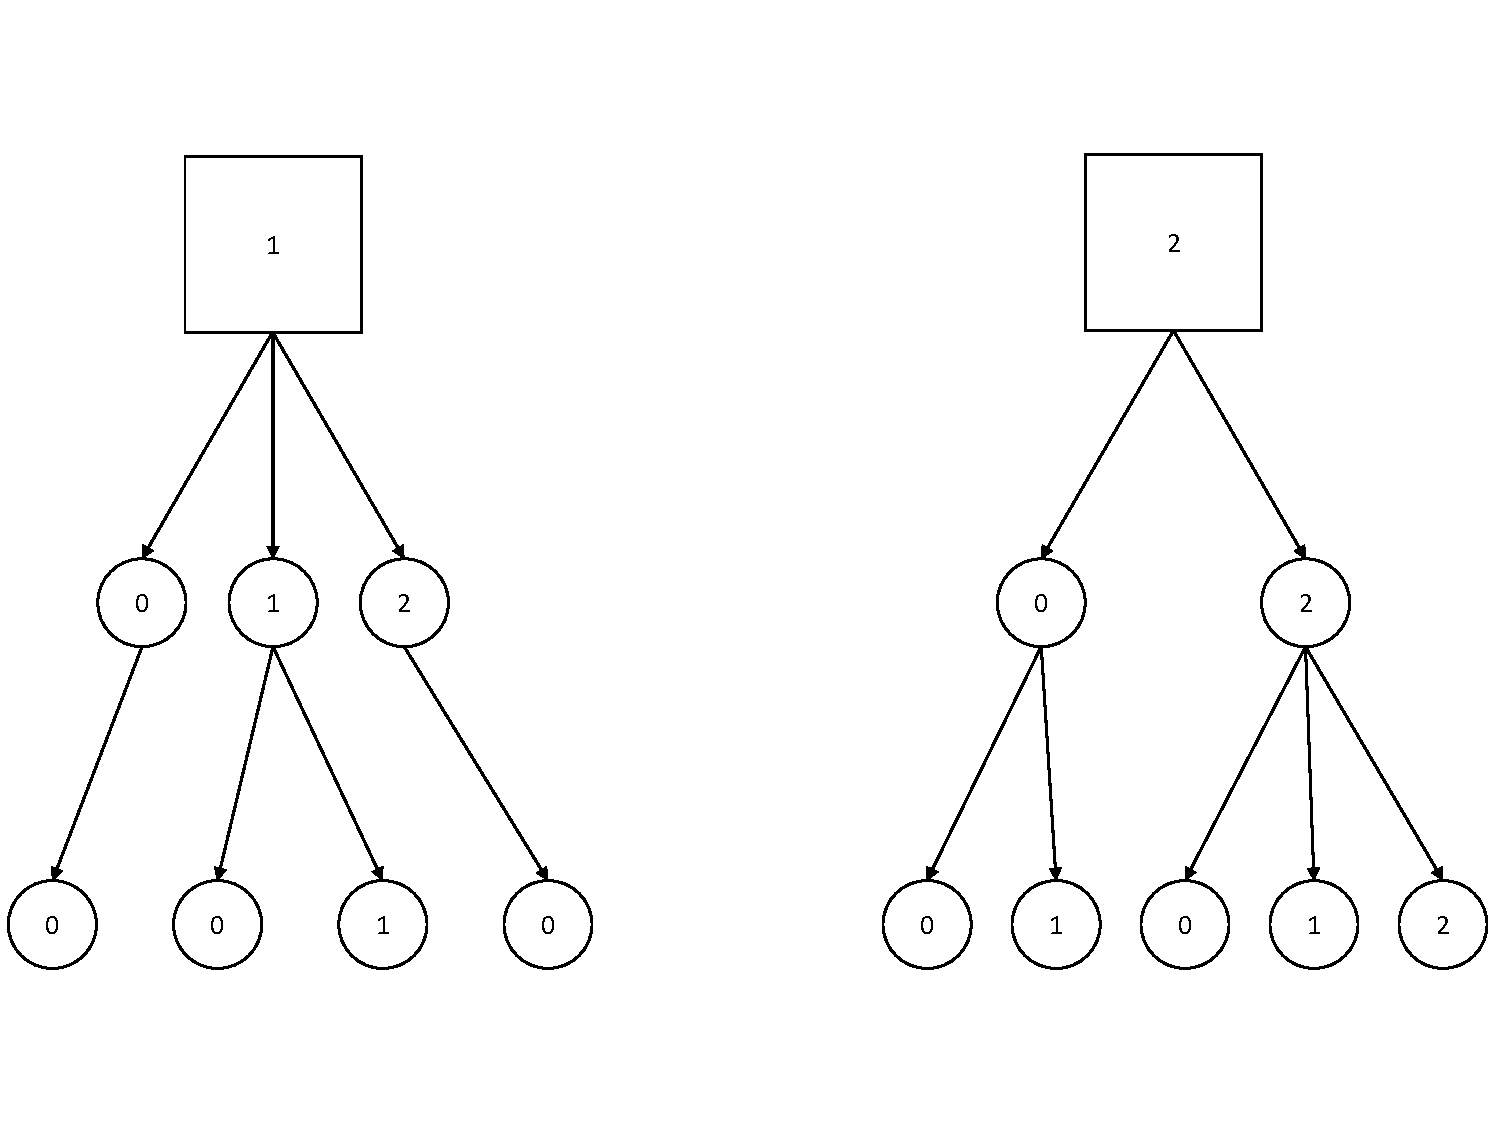
\includegraphics[clip, trim=0cm 2.5cm 0cm 2.5cm, width = .7\textwidth]{Track-tree}
\caption{Track hypothesis tree}
\label{fig:hyp-tree}
\end{figure}

\begin{equation}
\begin{split}
\M{A_1} &=\begin{bmatrix}
		0 & 1 & 1 & 0 & 0 & 0 & 0 & 0 & 0 \\
       	0 & 0 & 1 & 0 & 0 & 1 & 0 & 1 & 0 \\
       	0 & 0 & 0 & 1 & 0 & 0 & 1 & 1 & 1 \\
       	0 & 0 & 0 & 0 & 0 & 0 & 0 & 0 & 1 \\
     	\end{bmatrix}
\V{b_1} = 	\begin{bmatrix}
			1 \\ 1  \\ 1 \\ 1
			\end{bmatrix} \\
\M{A_2} &=\begin{bmatrix}
		1 & 1 & 1 & 1 & 0 & 0 & 0 & 0 & 0 \\
       	0 & 0 & 0 & 0 & 1 & 1 & 1 & 1 & 1 \\
     	\end{bmatrix} 
\V{b_2} = 	\begin{bmatrix}
			1 \\ 1
			\end{bmatrix} \\
\V{c} &=\begin{bmatrix}
		\lambda_1 & \lambda_2 & \lambda_3 & \lambda_4 & \lambda_5 & \lambda_6 & \lambda_7 & \lambda_8 & \lambda_9
		\end{bmatrix}^T \\
\end{split}
\label{eq:example_matrices}
\end{equation}

The explicit enumeration that becomes necessary when creating these $\M{A}$ matrices is exhaustive since dimension of $\V{\tau}$, which is equal to the number of leaf nodes in the track forest, can be very large. Both $\M{A}_1$ and $\M{A}_2$ grows quadratically with the number of track hypotheses and real measurements or number of targets respectively.
% $N_1$ is proportional with the number of targets and history steps (N-scan). 

\subsection{Solvers}
There are a lot of of-the-shelf \gls{ilp} and \gls{milp} solvers on the marked, both free open source and commercial. Since our problem is formulated on standard form, it can easily be executed on several solvers, and we can compare runtime and performance. In this report, the following solvers are tested:
\begin{itemize}
\item CBC 		(Free, COIN-OR)
\item CPLEX 	(Commercial (Free academic),  IBM)
\item GLPK 		(Free, GNU)
\item Gurobi 	(Commercial (Free academic), Gurobi)
\end{itemize}
	%!TEX root = ../TTK4550-MHT.tex
\section{Results}
\label{sec:results}

\subsection{Testing scheme}
The evaluation of the \gls{mht} algorithm is two-sided. Firstly the algorithm must be able to track under challenging conditions, and secondly it must be able to do so without having an ever growing computational cost and run time. The first performance metric is how well the algorithm is estimating the true position to the object it is tracking. We measure this by means of the Euclidean distance between the estimated and true track (\ref{eq:euclidian_distance_vector}).
\begin{equation}
	\Delta P = \| \V{p}_{track}-\V{p}_{target} \|_2
\label{eq:euclidian_distance_vector}
\end{equation}
The track is considered correct if $\Delta P \leq \varepsilon_p$ for all t after initial convergence. If a track is deviating more than the threshold and never return within the threshold again, it is considered lost at the time-step when it exceeded the threshold. If the track should converge after exceeding the threshold, it is considered restored at the time-step it is returning within the limit. 

The algorithm is tested on six scenarios:
\begin{itemize}
	\item Five fully cooperating ships
    \item Five partially cooperative ships
    \item Five ships avoiding obstacles with large space
    \item Five ships avoiding obstacles with little space
	\item Five almost parallel ships (normal speed \gls{radar})
	\item Five almost parallel ships (high speed \gls{radar})
\end{itemize}
\begin{figure}[H]
    \centering
    \begin{subfigure}{0.45\textwidth}
        \centering
        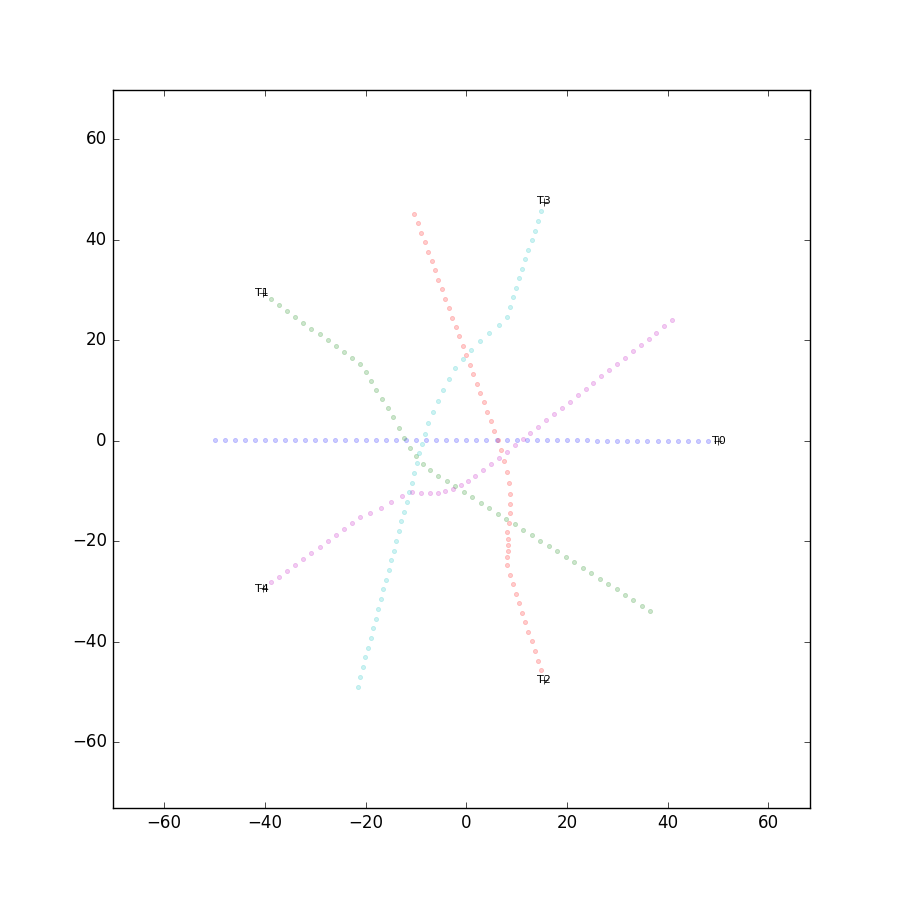
\includegraphics[height=0.27\textheight]{scenario1}
        \caption{First scenario}
    \end{subfigure}
    \begin{subfigure}{0.45\textwidth}
        \centering
        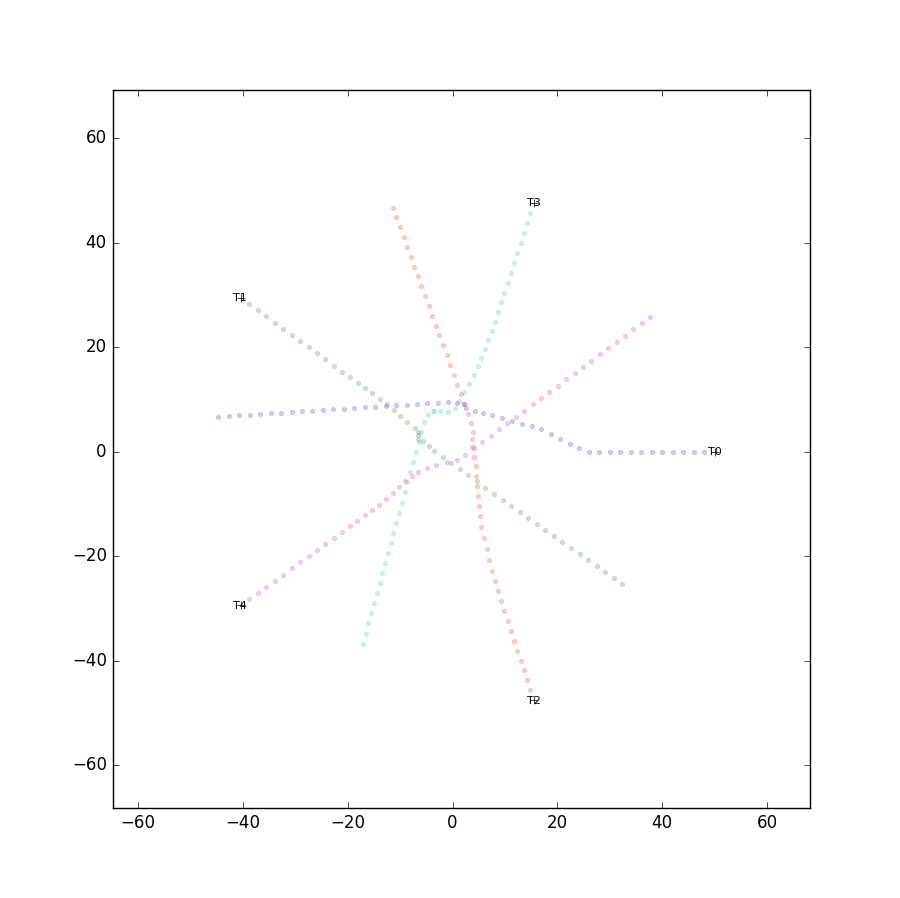
\includegraphics[height=0.27\textheight]{scenario2}
        \caption{Second scenario}
    \end{subfigure}
    \begin{subfigure}{0.45\textwidth}
        \centering
        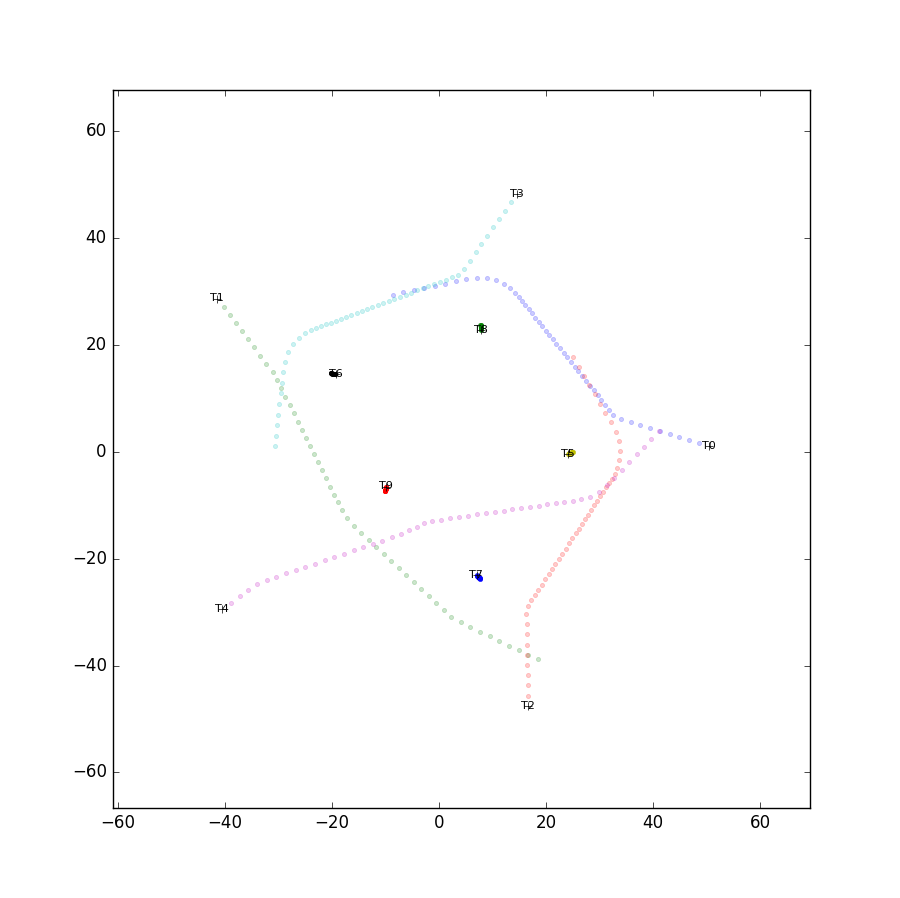
\includegraphics[height=0.27\textheight]{scenario3}
        \caption{Third scenario}
    \end{subfigure}
    \begin{subfigure}{0.45\textwidth}
        \centering
        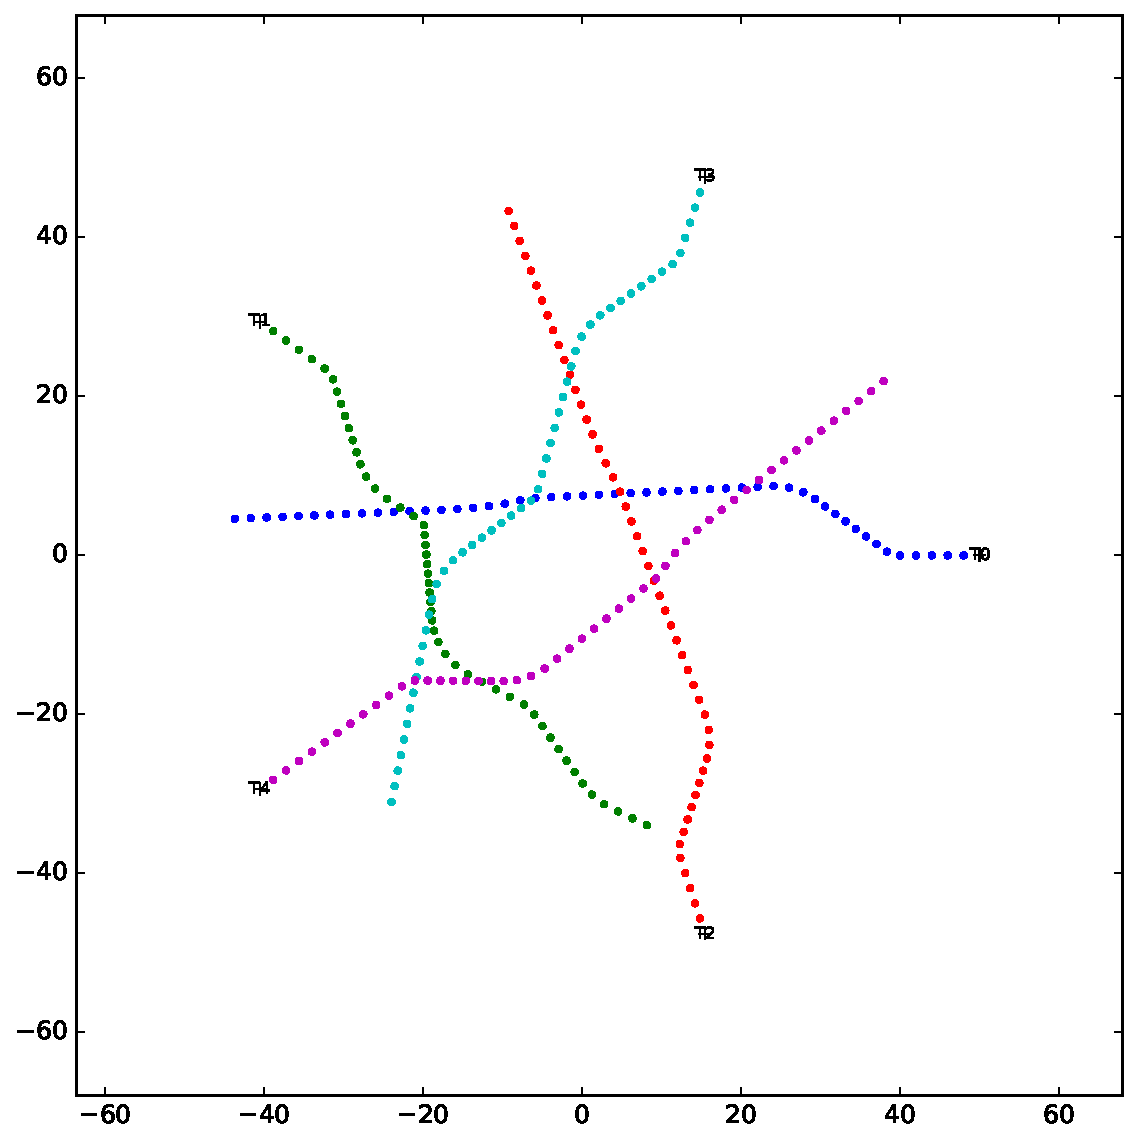
\includegraphics[height=0.27\textheight]{scenario4}
        \caption{Fourth scenario}
    \end{subfigure}
    \begin{subfigure}{0.45\textwidth}
        \centering
        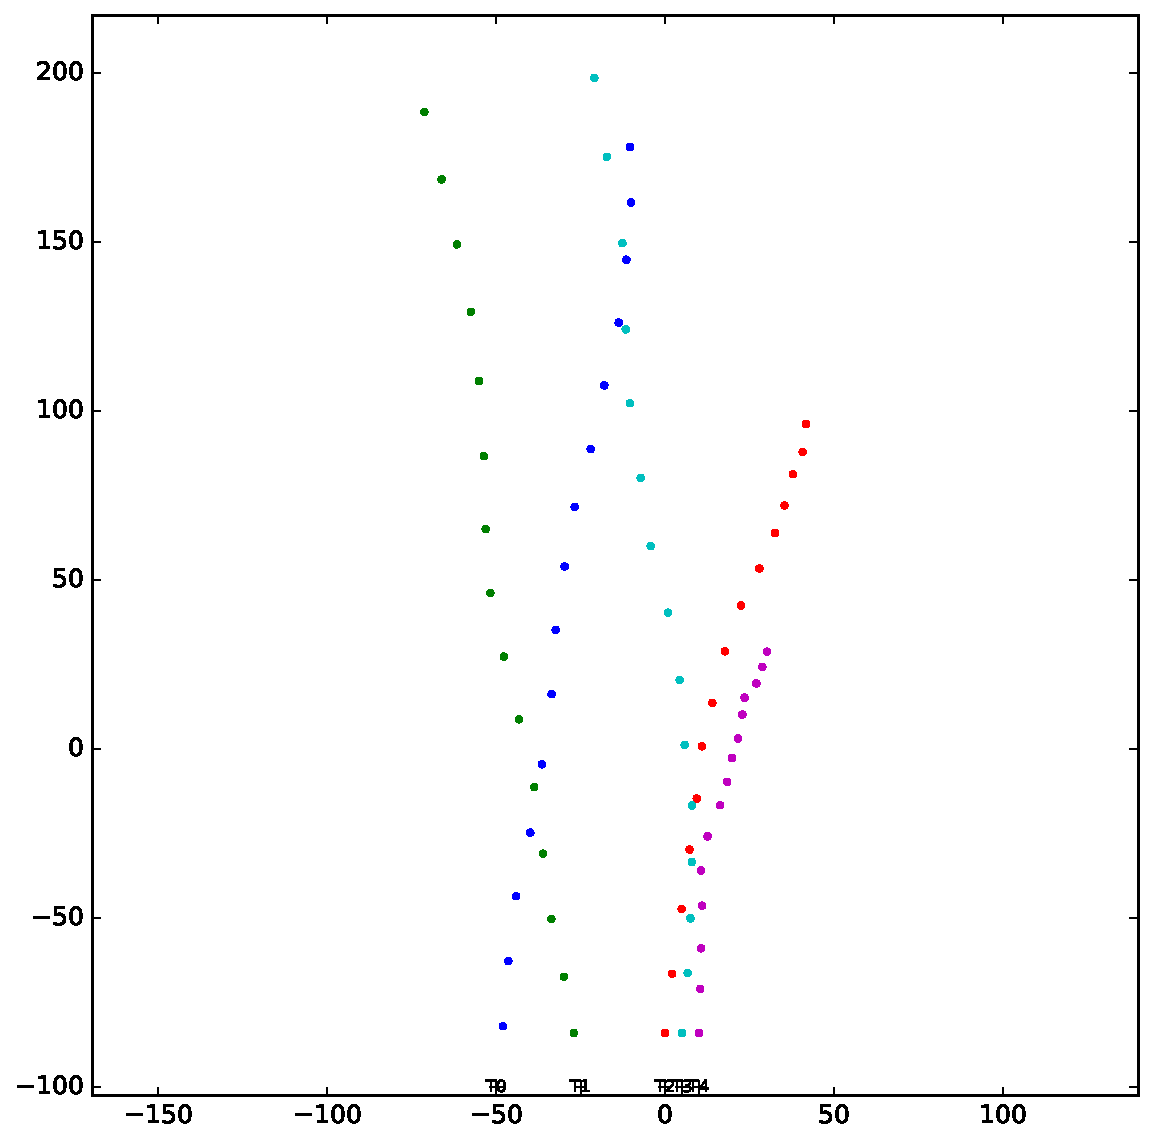
\includegraphics[height=0.27\textheight]{scenario5}
        \caption{Fifth scenario}
    \end{subfigure}
    \begin{subfigure}{0.45\textwidth}
        \centering
        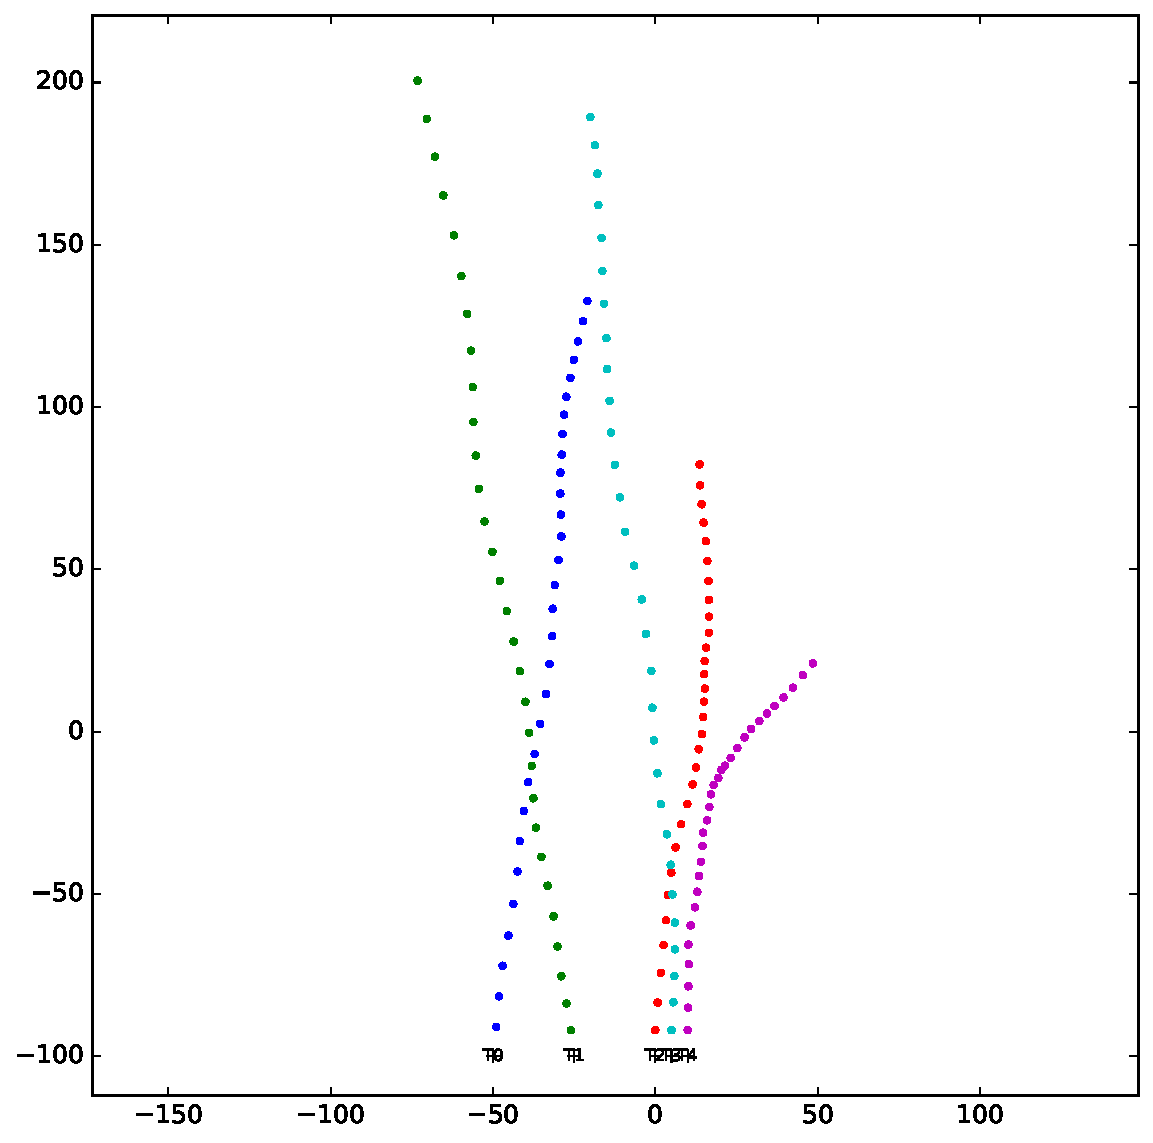
\includegraphics[height=0.27\textheight]{scenario6}
        \caption{Sixth scenario}
    \end{subfigure}
    \caption{True track for scenario 1-6}
    \label{fig:true_tracks}
\end{figure} 

\subsection{Simulation data}
Scenario one through four was generated as a recording of time and position from an \gls{asv} simulator with \gls{colav}, developed by Dr. D. Kwame Minde  Kufolaor at \gls{ntnu}. The ships are configured such that they need to maneuver to avoid collision with each other, which allows for tracking of maneuvering targets in close proximity to each other. These scenarios where sampled at 1 Hz which is a little faster than a normal high speed vessel \gls{radar} at 0.8 Hz (48 \gls{rpm}). The fifth and sixth scenario was generated as a part of this project, and is composed by linear parallel paths with white Gaussian system noise as maneuvering. These scenarios were sampled from the same data set at 0.5 Hz  and 1 Hz respectively, where 0.5 Hz is a little higher that a normal maritime coastal \gls{radar} at 0.4 Hz (24 \gls{rpm}). The usage of two different sample rates were to compare the most common \gls{radar} update frequencies used in the maritime sector with respect to tracking performance. The different ranges, \gls{fov}, and expected clutter points for the different scenarios are summarized in Table \ref{tab:clutter_measurements}.

\begin{table}
\centering
\begin{tabular}{c c c c c c c c}
			&				&						& & &$\lambda_\phi \cdot FOV$& 	&		\\
Scenario 	& Radar range	& \gls{fov}				& $1$ 	& $2$ 	& $4$ 	&$6$ 	& $8$	\\ \hline
1-4		 	& $65 m$ 		& $1.3\cdot10^4 m^2$	& 1.3 	& 2.6 	& 5.2 	& 7.38 	& 9.21 	\\
5-6		 	& $155 m$		& $7.5\cdot10^4 m^2$	& 3.22 	& 4.61 	& 5.99 	& 7.38 	& 9.21 					
\end{tabular}
\caption{Expected number of clutter measurements in scenarios}
\label{tab:clutter_measurements}
\end{table}

\subsection{Simulations}
Scenario one through six was simulated with the following variations with all four solvers.
\begin{equation*}
\begin{split}
\V{P_D} &= \begin{bmatrix} 0.5 & 0.6 & 0.7 & 0.8 & 0.9 \end{bmatrix} \\
\V{N} &=\begin{bmatrix} 0 & 1 & 3 & 6 & 9 \end{bmatrix} \\
\V{\lambda_\phi} &=\begin{bmatrix} 0 & 1\cdot10^{-4} & 2\cdot10^{-4} & 4\cdot10^{-4} & 6\cdot10^{-4} & 8\cdot10^{-4} \end{bmatrix}
\end{split}
\end{equation*}
Each of the 3600 variants was simulated 160 times with different seeded random clutter measurements and misdetections. These simulations required approximately 864 \gls{cpu} hours, and were for the most part simulated on a 36 core virtualized server. For each simulation, the estimated tracks were compared with the true tacks and categorised in successful and lost tracks, where the track loss threshold $\epsilon_p$ was $4$ meters. Figure \ref{fig:track_hypotheses_example} display a mid-simulation plot with current best tracks in solid lines, and hypotheses in dotted lines. Notice how many of the hypotheses have very similar paths, and with a certain margin duplicates each other.
\begin{figure}[H]
    \centering
    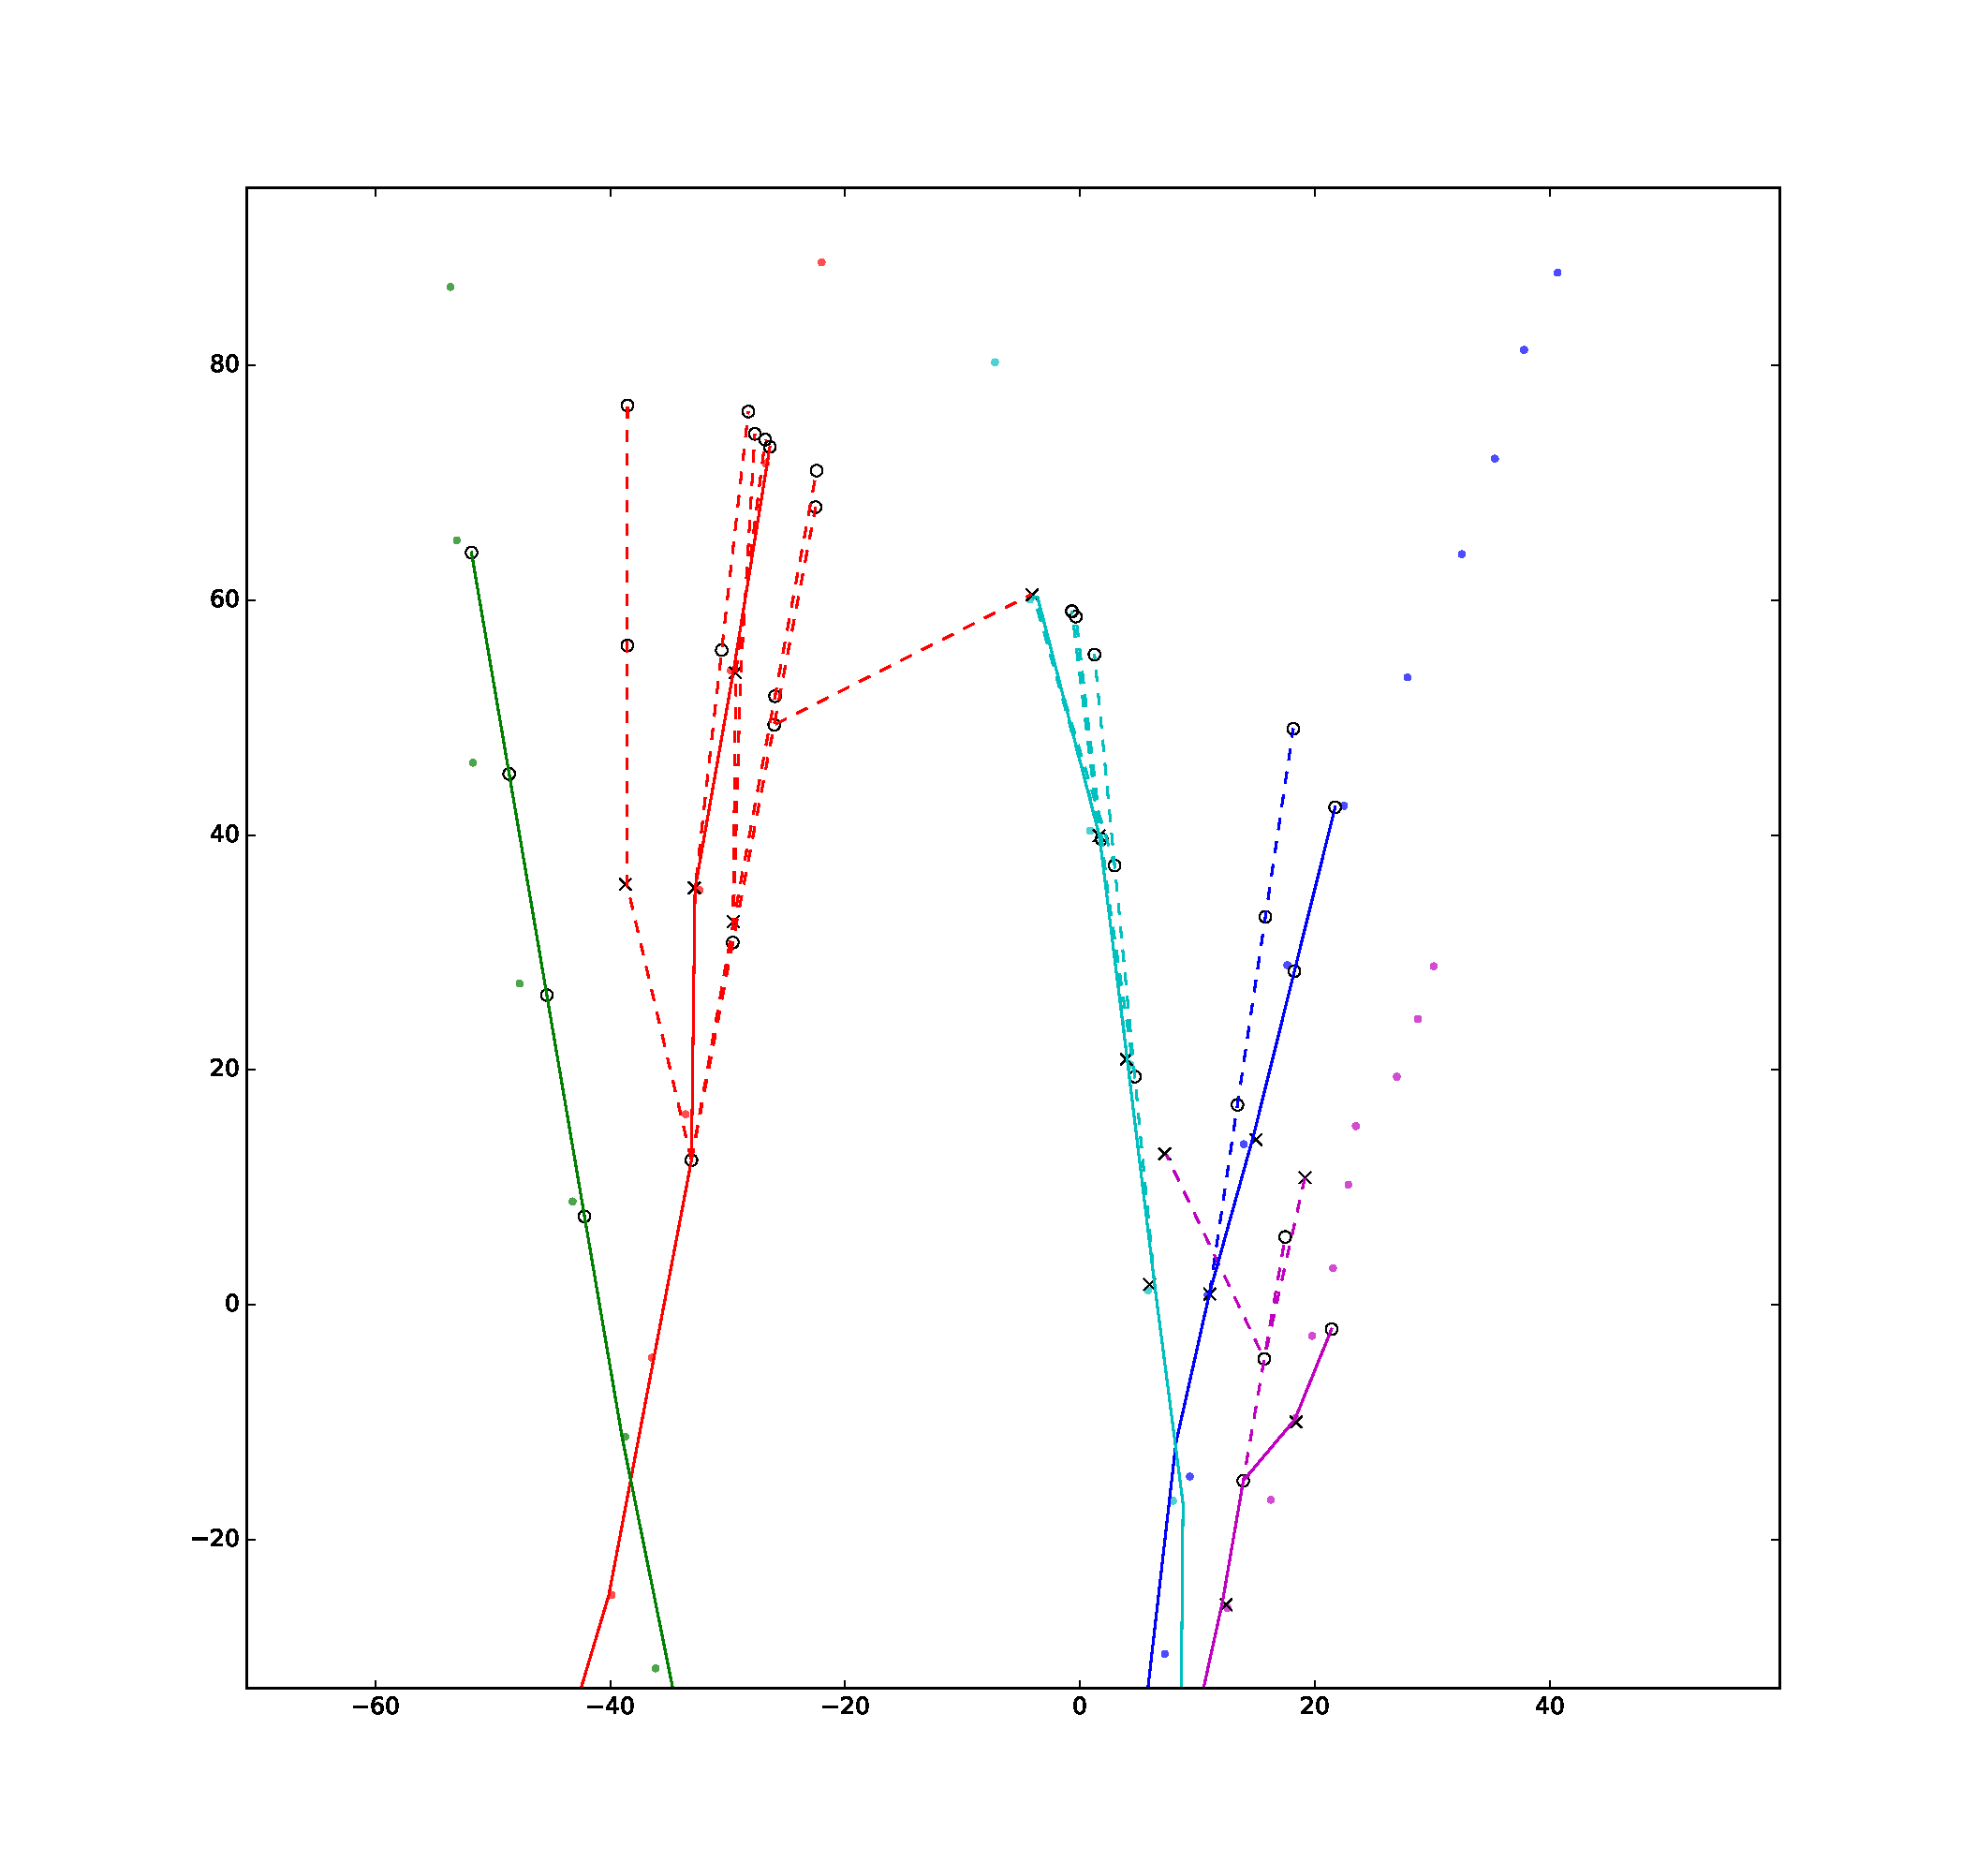
\includegraphics[clip, trim=3cm 2.5cm 3cm 3cm,width=0.7\textwidth]{tracks_with_hypotheses}
    \caption{Track hypotheses example}
    \label{fig:track_hypotheses_example}
\end{figure}
Figure \ref{fig:tracking_performance} shows the track performance from the "GLPK" solver. The performance of the other solvers can be found in the appendix, Figures \ref{fig:dynamic_agents_full_cooperation_cropped} - \ref{fig:dynamic_and_static_agents_narrow_space_cropped}.
\begin{figure}[H]
    \centering
    \begin{subfigure}{0.49\textwidth} 
        \centering
        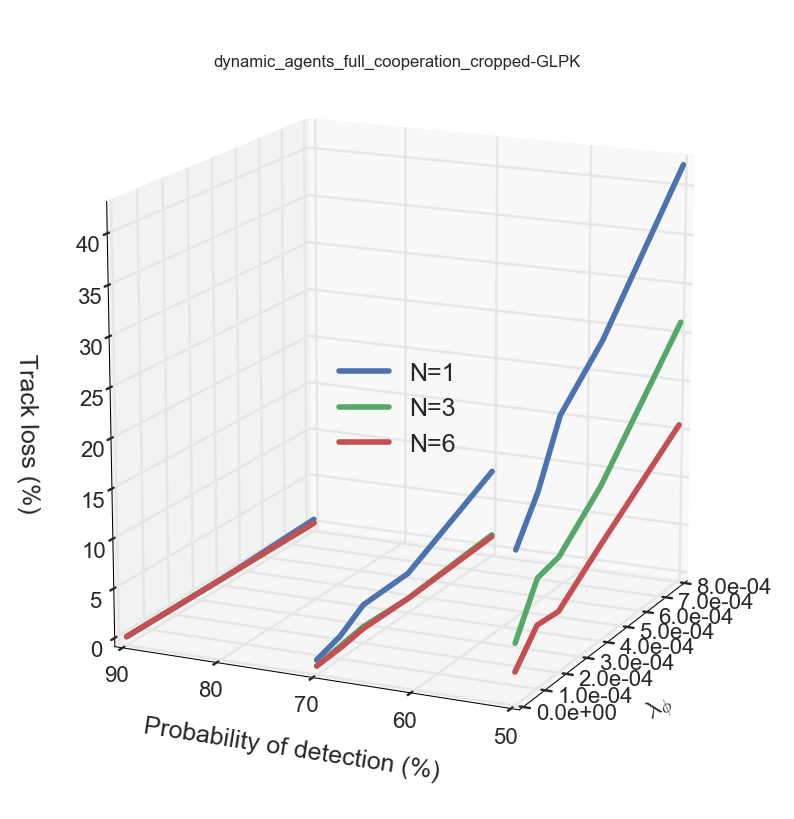
\includegraphics[clip, trim=0cm 1cm 0cm 1cm, height=0.28\textheight]{dynamic_agents_full_cooperation_cropped-GLPK}
        \caption{Scenario 1}
    \end{subfigure}
    \begin{subfigure}{0.49\textwidth}
        \centering
        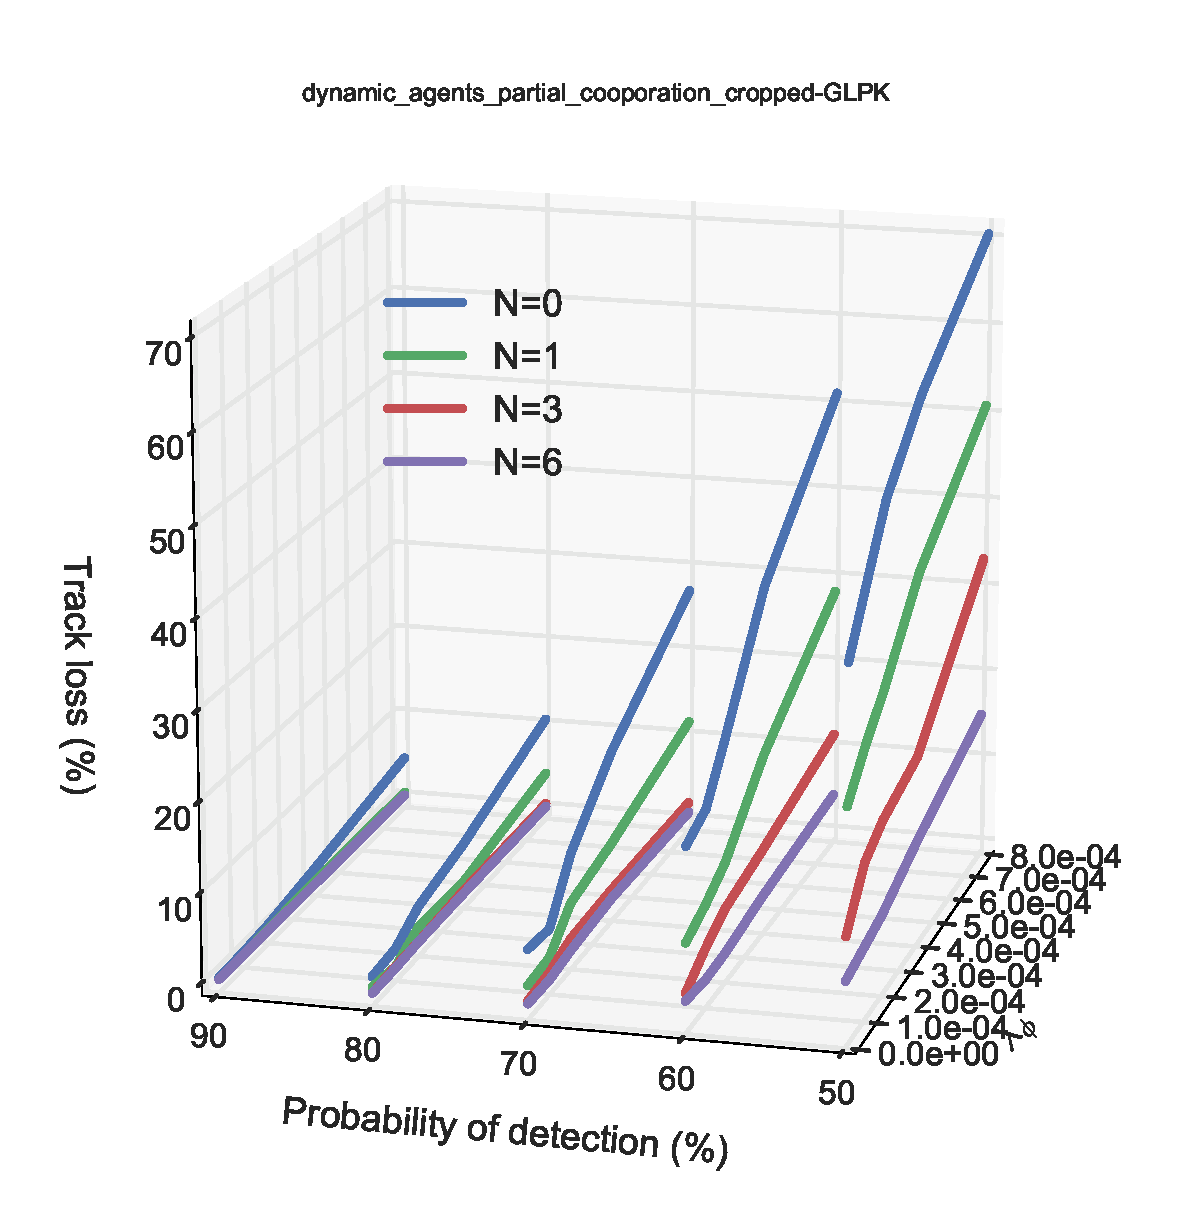
\includegraphics[clip,  trim=0cm 1cm 0cm 1cm,height=0.28\textheight]{dynamic_agents_partial_cooporation_cropped-GLPK}
        \caption{Scenario 2}
    \end{subfigure}
    \begin{subfigure}{0.49\textwidth}
        \centering
        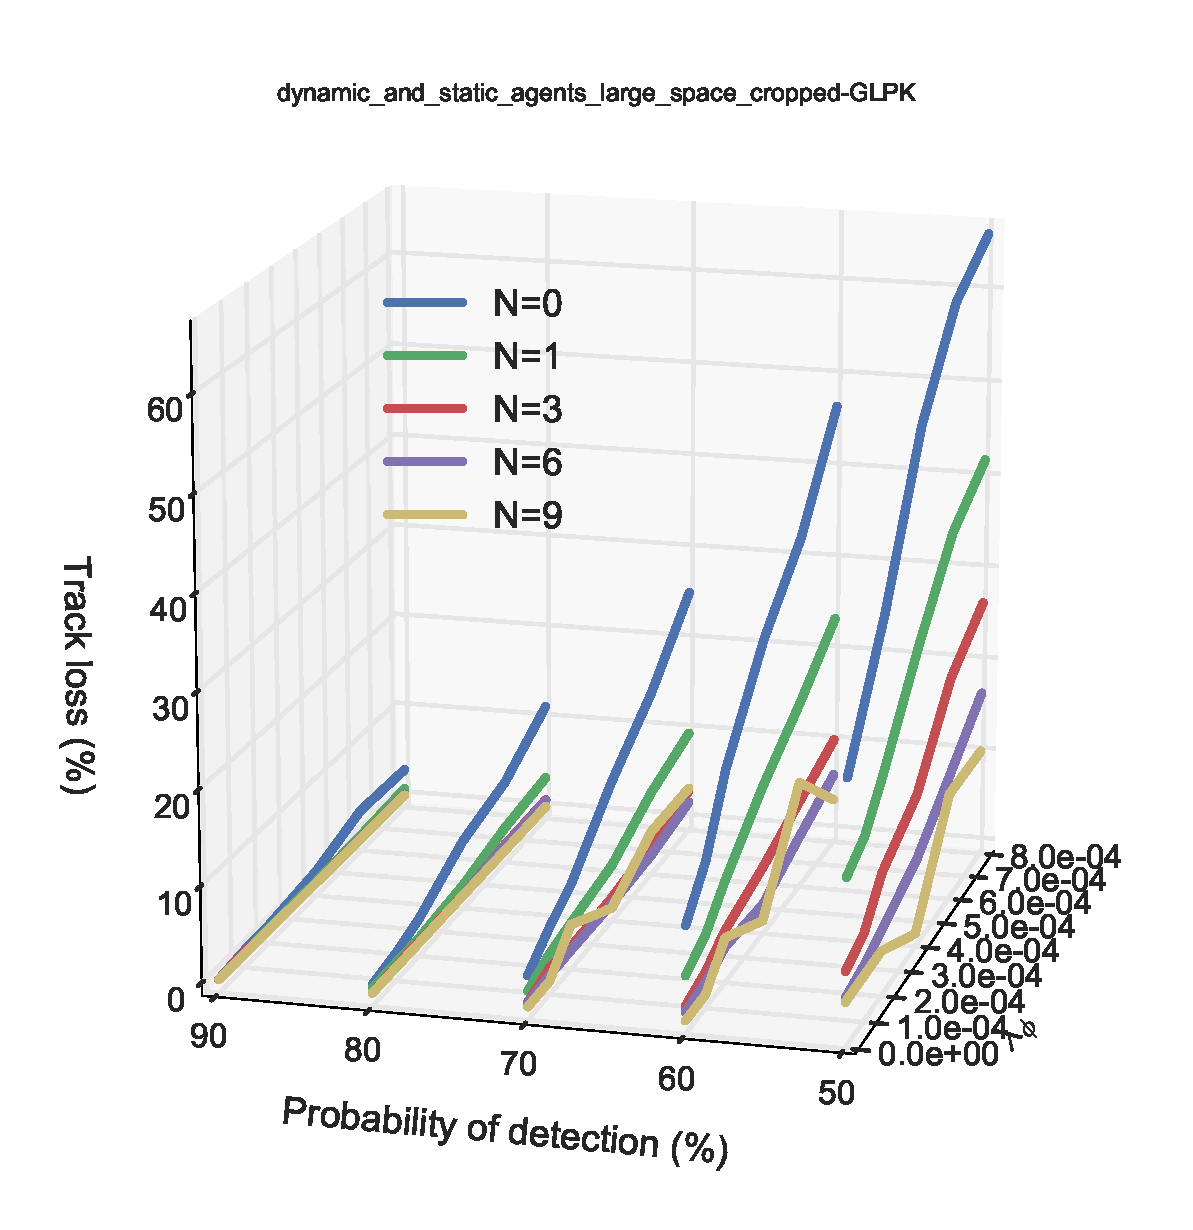
\includegraphics[clip,  trim=0cm 1cm 0cm 1cm,height=0.28\textheight]{dynamic_and_static_agents_large_space_cropped-GLPK}
        \caption{Scenario 3}
    \end{subfigure}
    \begin{subfigure}{0.49\textwidth}
        \centering
        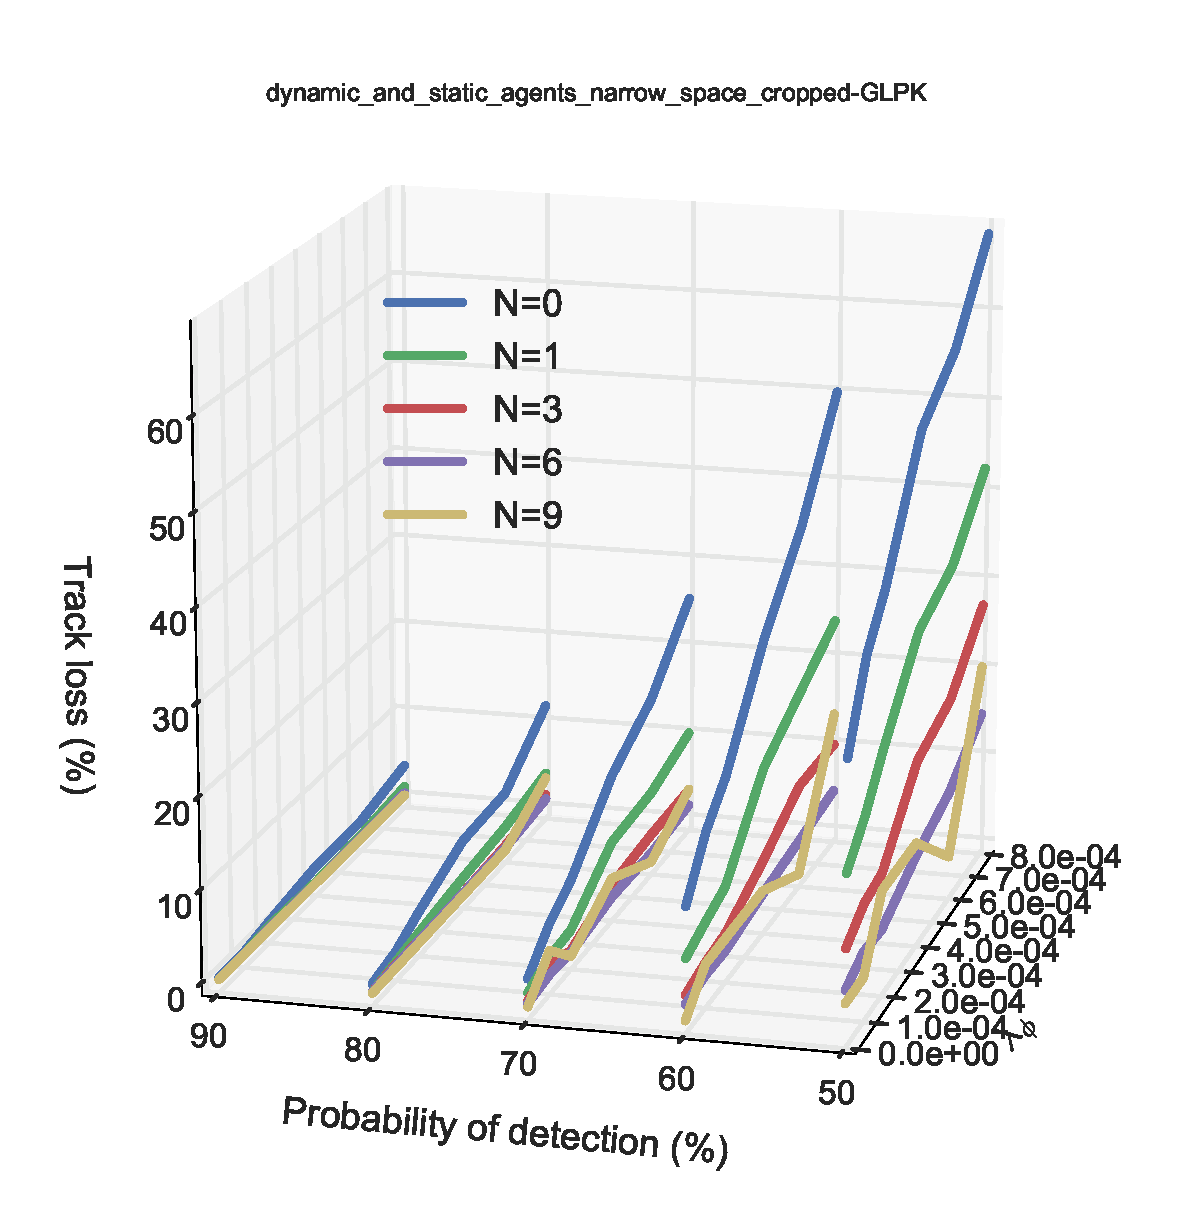
\includegraphics[clip,  trim=0cm 1cm 0cm 1cm,height=0.28\textheight]{dynamic_and_static_agents_narrow_space_cropped-GLPK}
        \caption{Scenario 4}
    \end{subfigure}
     \begin{subfigure}{0.49\textwidth}
        \centering
        \includegraphics[clip,  trim=0cm 1cm 0cm 1cm,height=0.28\textheight]{{parallel_targets_0.5hz-GLPK}.pdf}
        \caption{Scenario 5}
    \end{subfigure}
     \begin{subfigure}{0.49\textwidth}
        \centering
        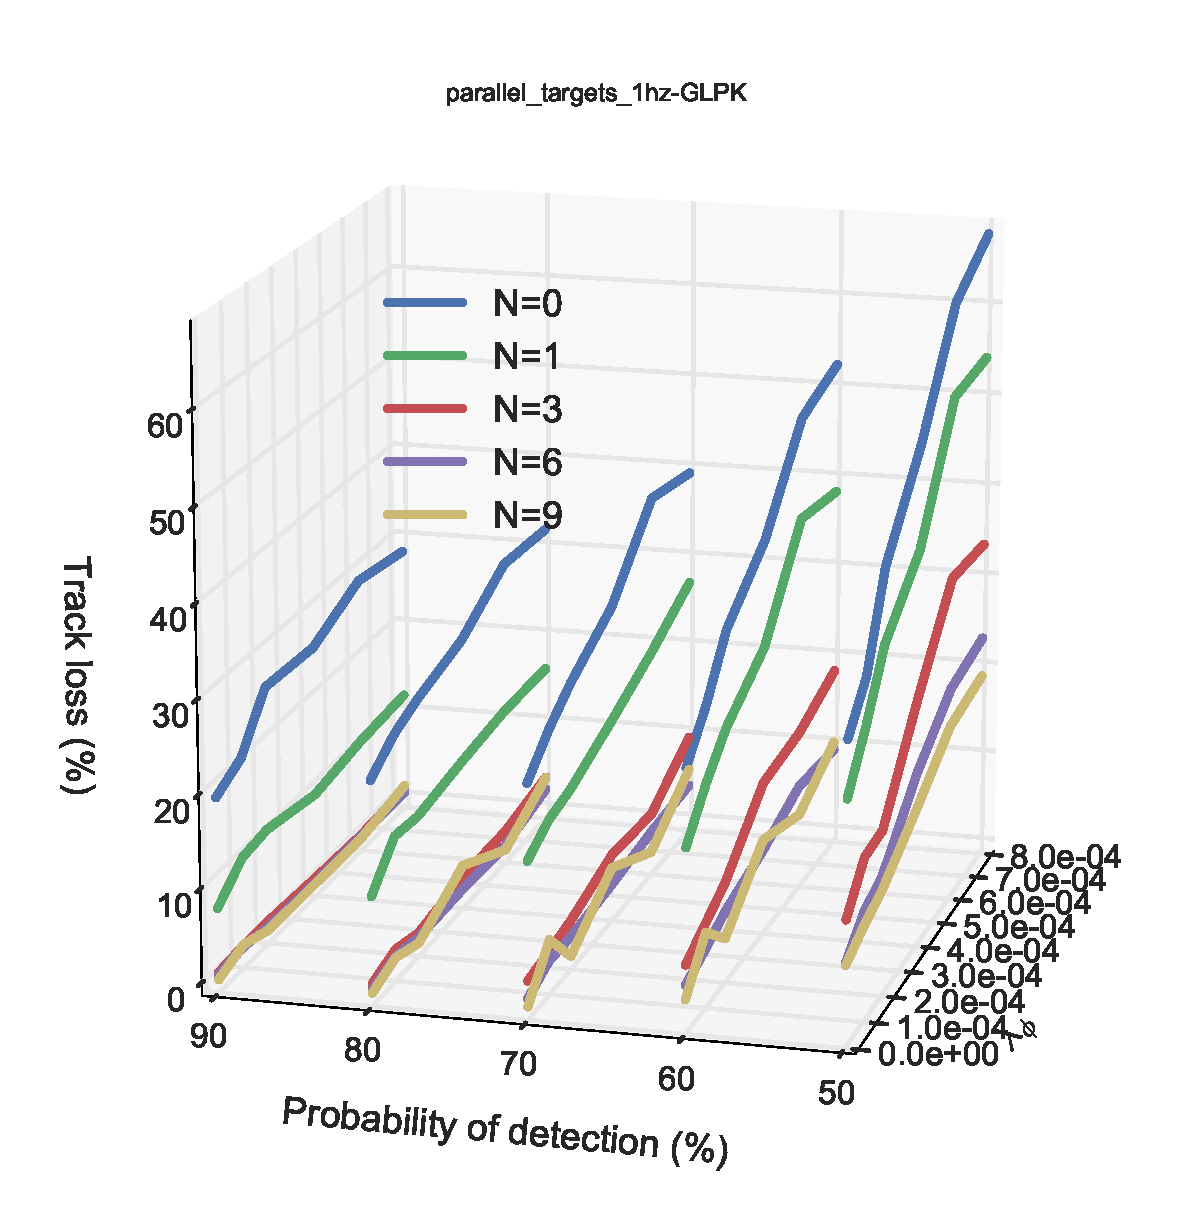
\includegraphics[clip,  trim=0cm 1cm 0cm 1cm,height=0.28\textheight]{parallel_targets_1hz-GLPK}
        \caption{Scenario 6}
    \end{subfigure}
	\caption{Simulation results for all scenarios}
    \label{fig:tracking_performance}
\end{figure}

\subsection{Runtime}
Figure \ref{fig:runtime_scenario_1} to \ref{fig:runtime_scenario_5} displays the average the runtime for the different solvers. The runtime along the z-axis displays the time used for simulating the entire scenario.

\begin{figure}[H]
\centering
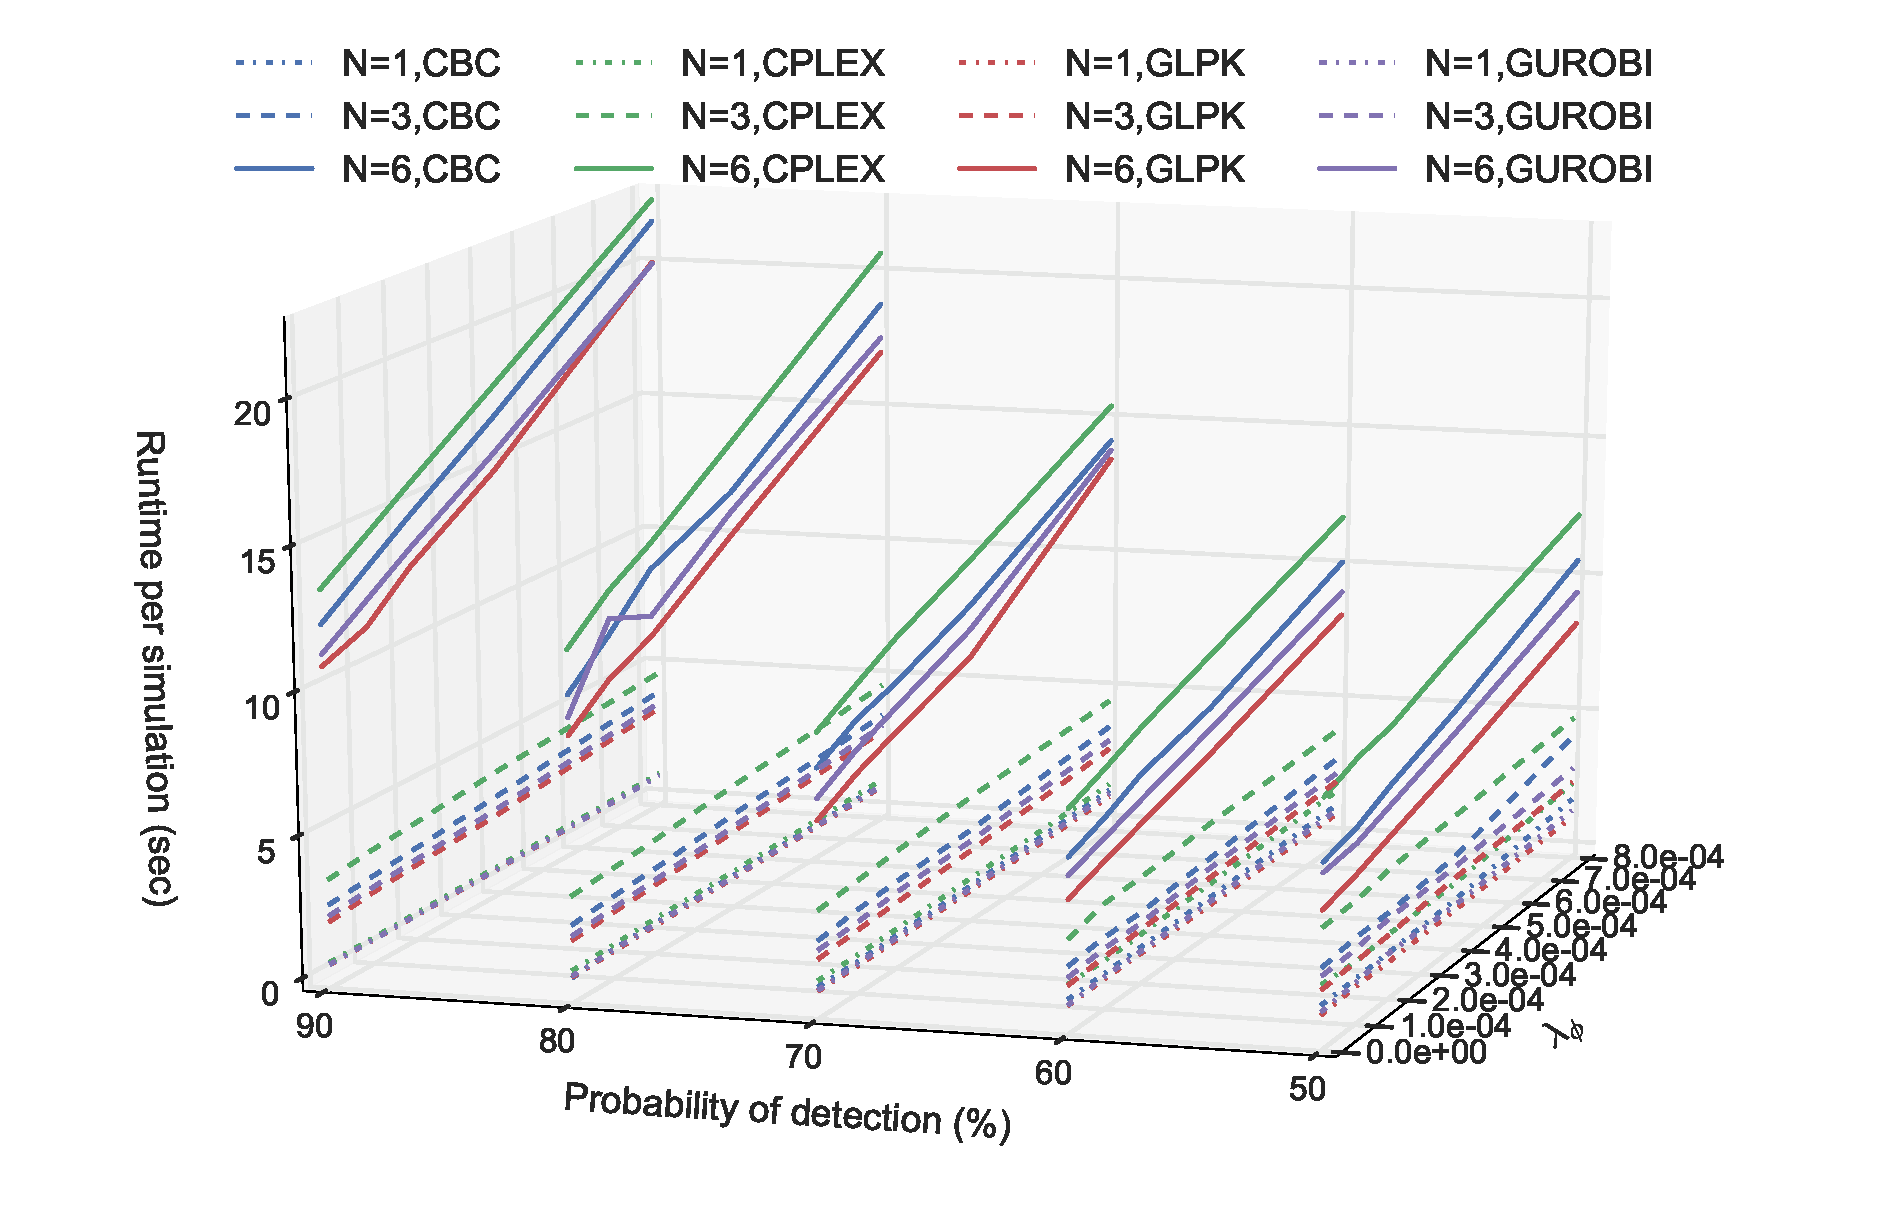
\includegraphics[clip, trim=0cm 1.5cm 0cm 0cm, width=\textwidth]{dynamic_agents_full_cooperation_cropped_runtime}
\caption{Runtime for scenario 1}
\label{fig:runtime_scenario_1}
\end{figure}

\begin{figure}[H]
\centering
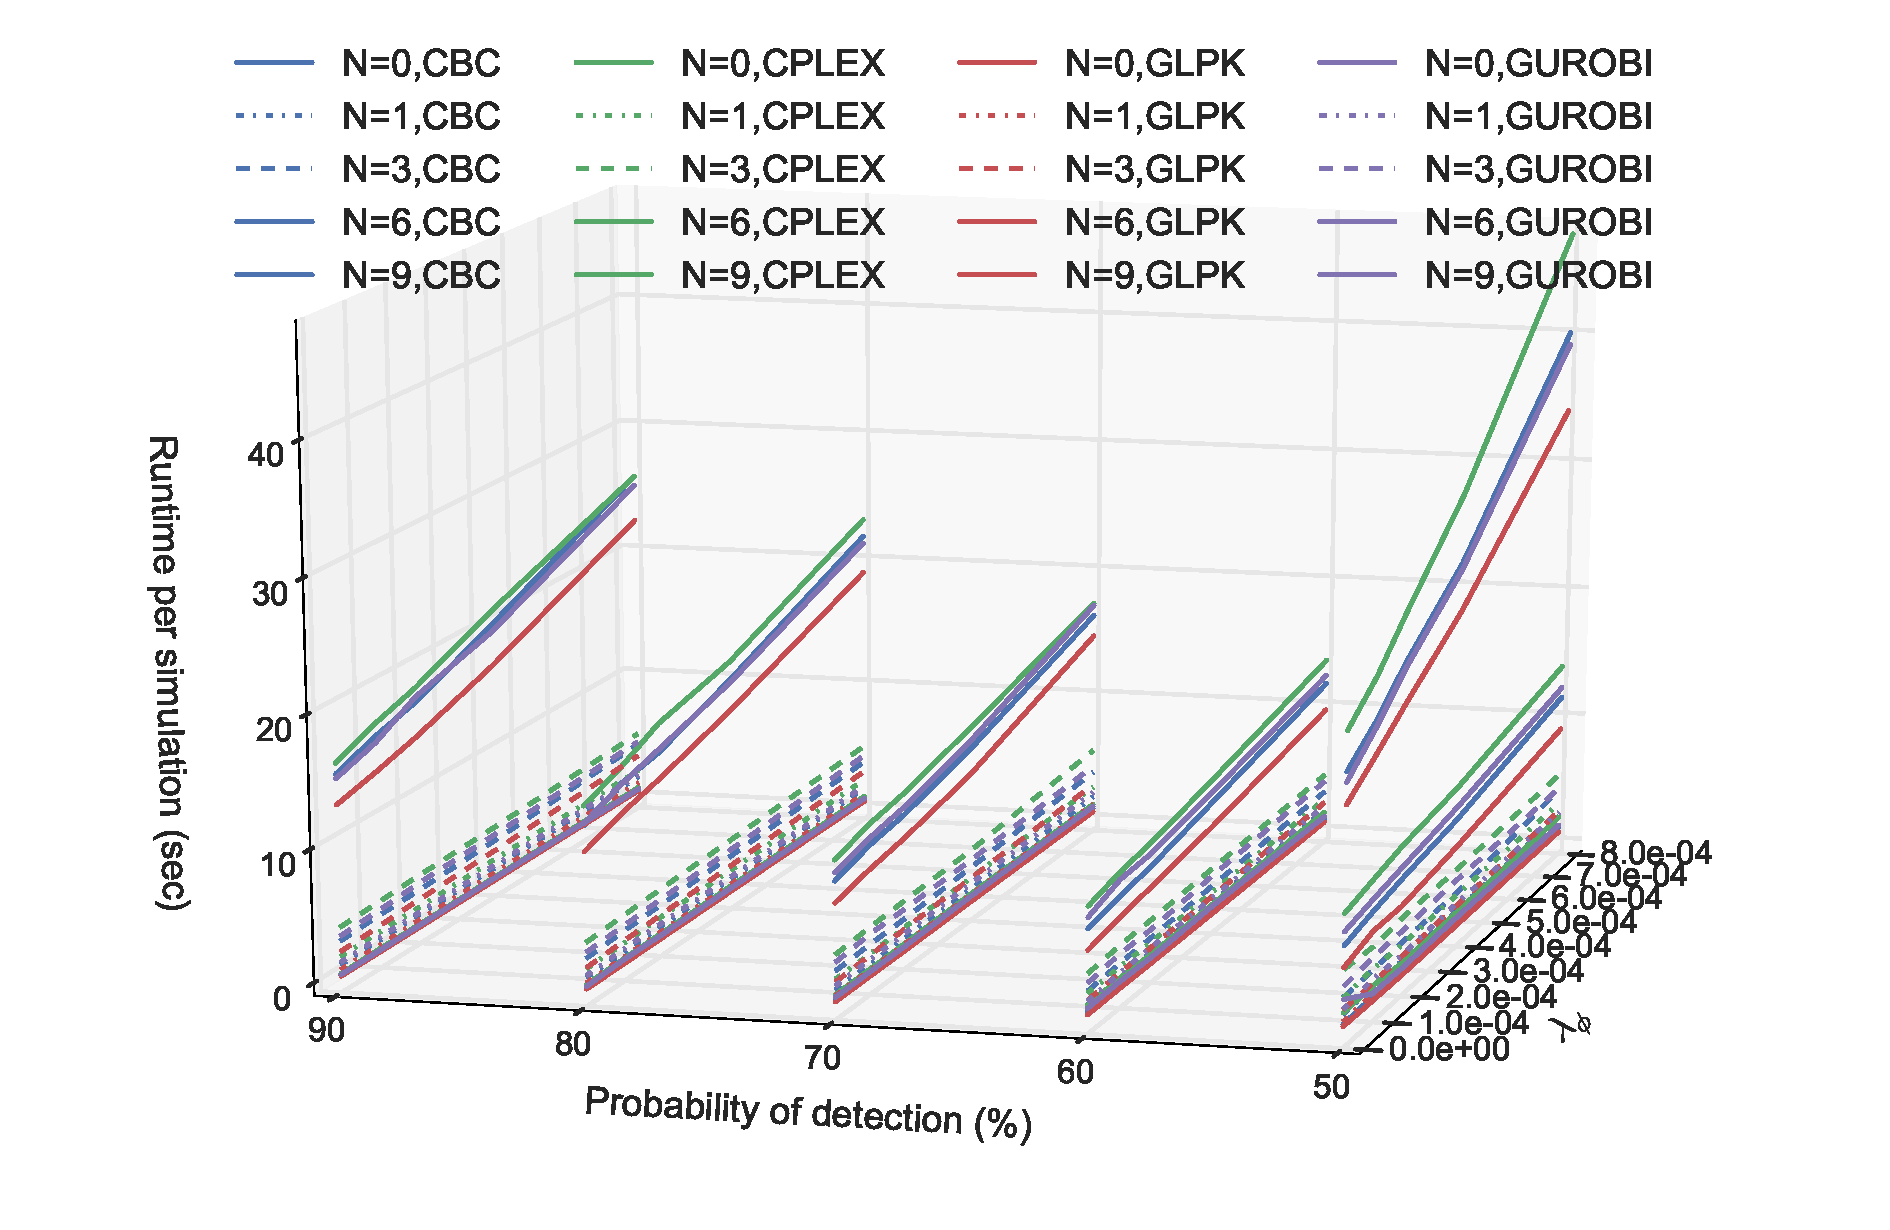
\includegraphics[clip, trim=0cm 1.5cm 0cm 0cm,width=\textwidth]{dynamic_agents_partial_cooporation_cropped_runtime}
\caption{Runtime for scenario 2}
\label{fig:runtime_scenario_2}
\end{figure}

\begin{figure}[H]
\centering
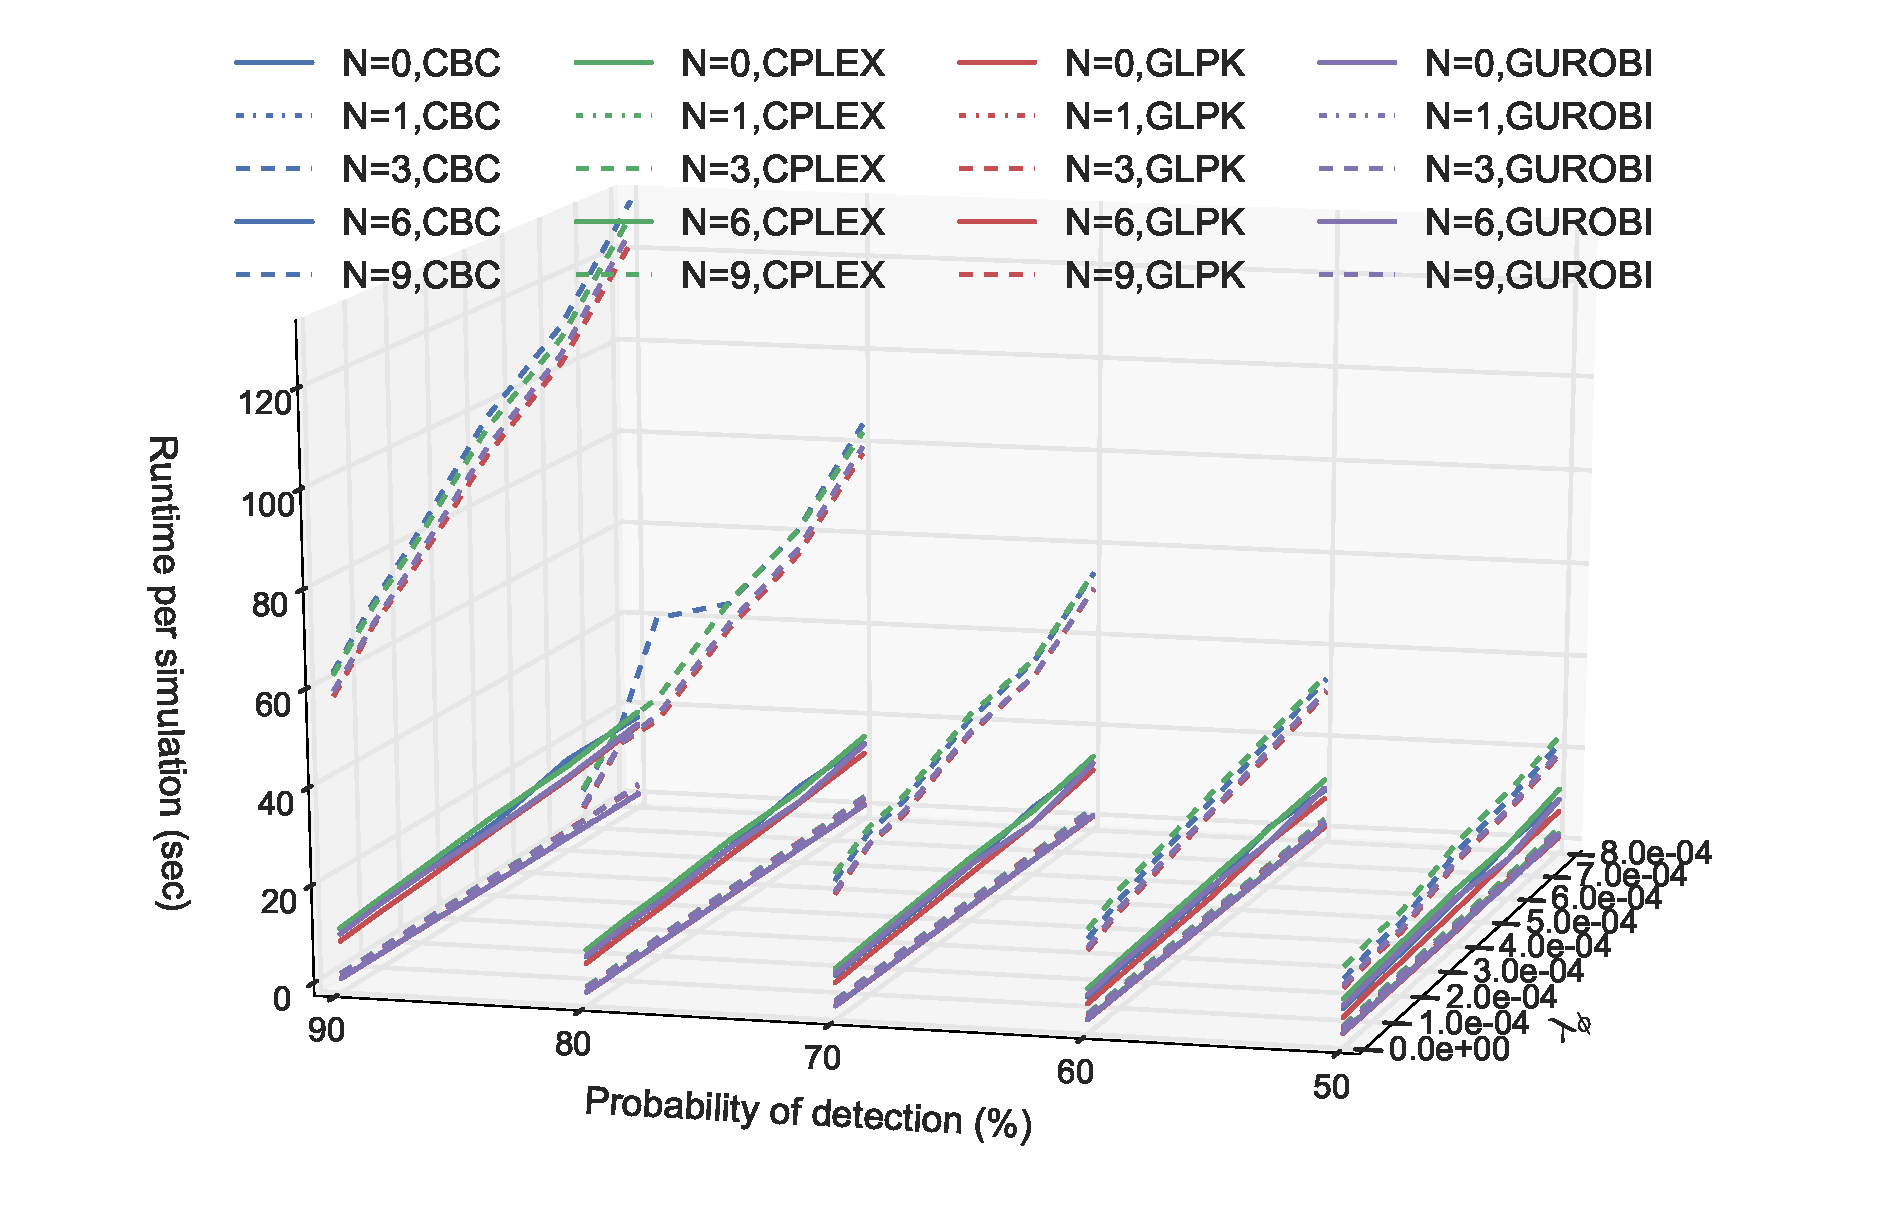
\includegraphics[clip, trim=0cm 1.5cm 0cm 0cm,width=\textwidth]{dynamic_and_static_agents_large_space_cropped_runtime}
\caption{Runtime for scenario 3}
\label{fig:runtime_scenario_3}
\end{figure}

\begin{figure}[H]
\centering
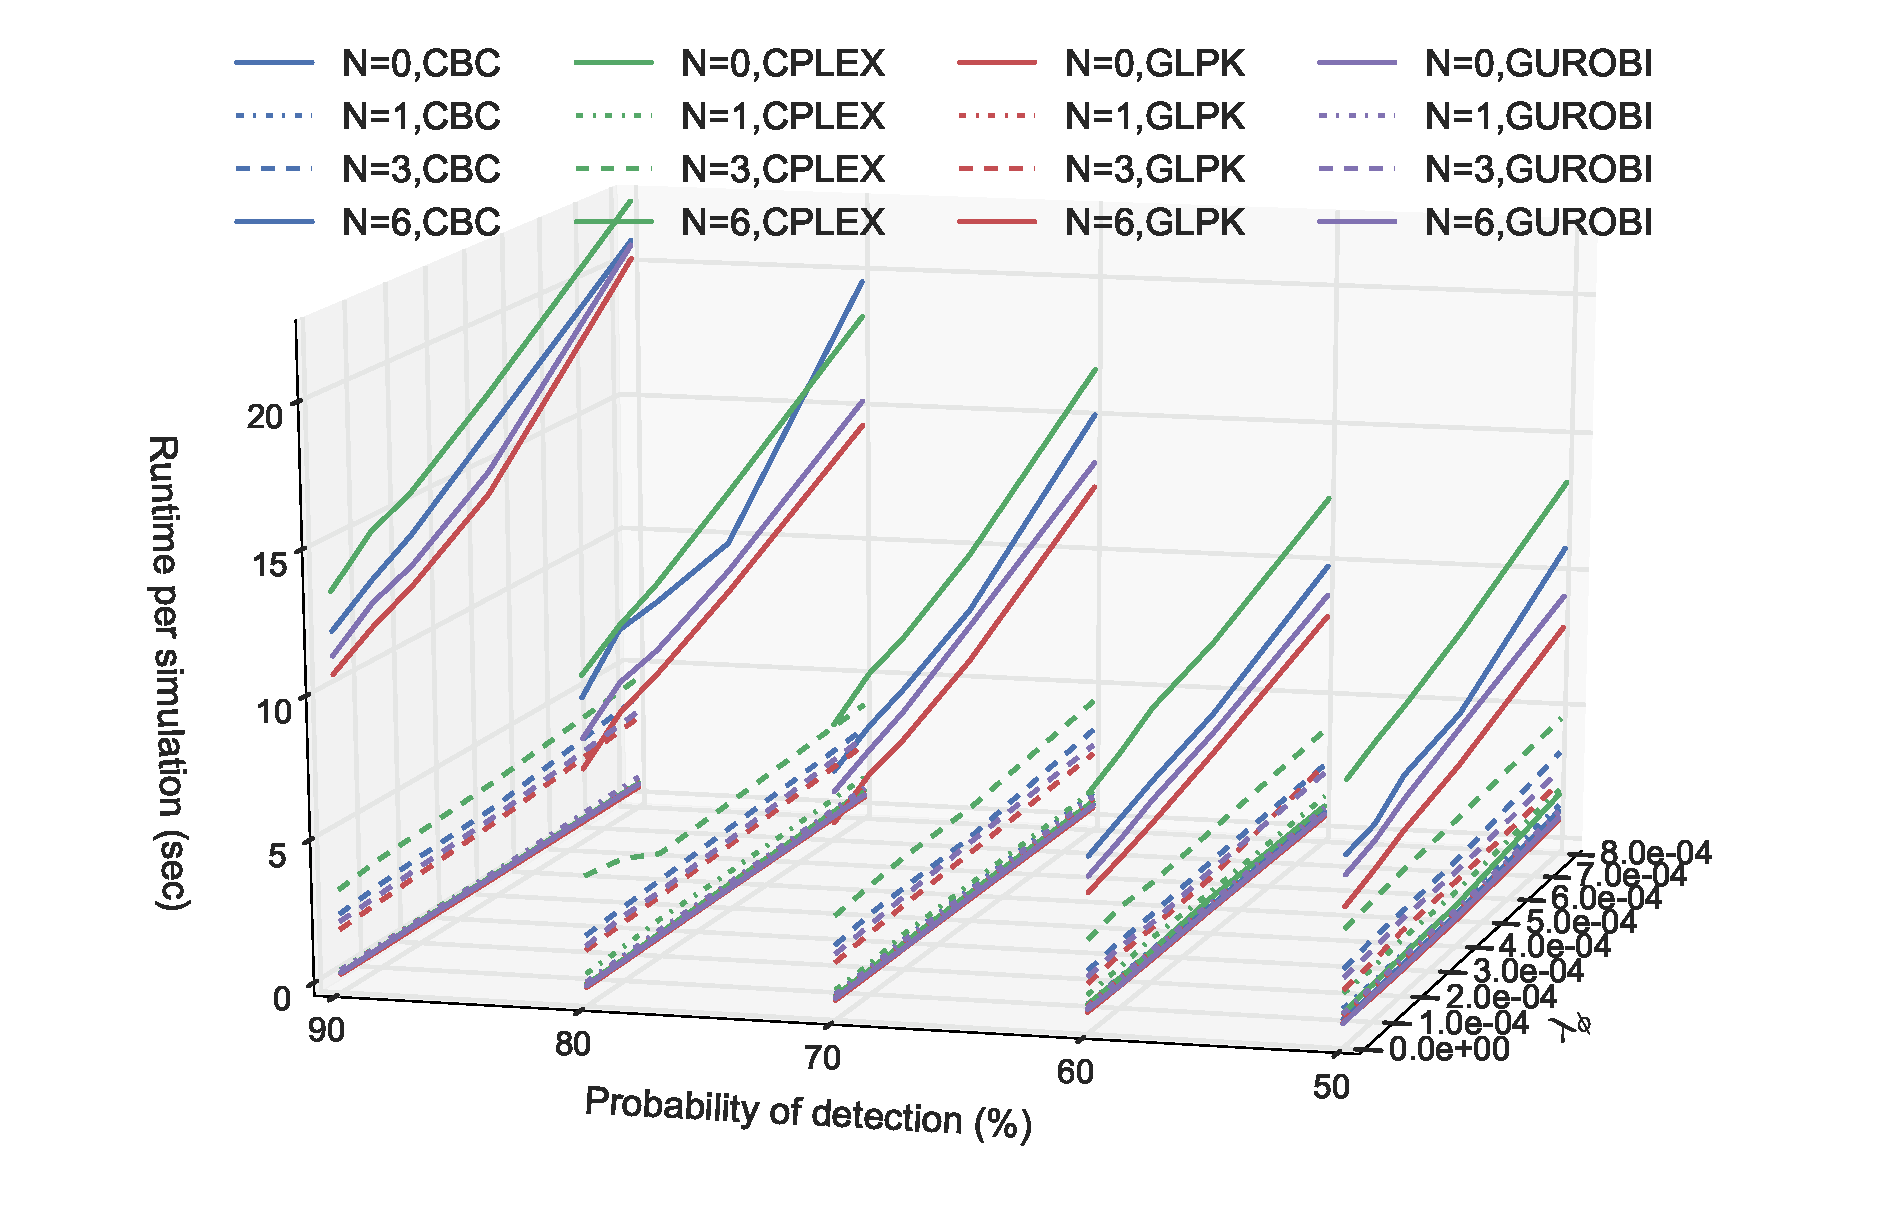
\includegraphics[clip, trim=0cm 1.5cm 0cm 0cm,width=\textwidth]{dynamic_and_static_agents_narrow_space_cropped_runtime}
\caption{Runtime for scenario 4}
\label{fig:runtime_scenario_4}
\end{figure}

\begin{figure}[H]
\centering
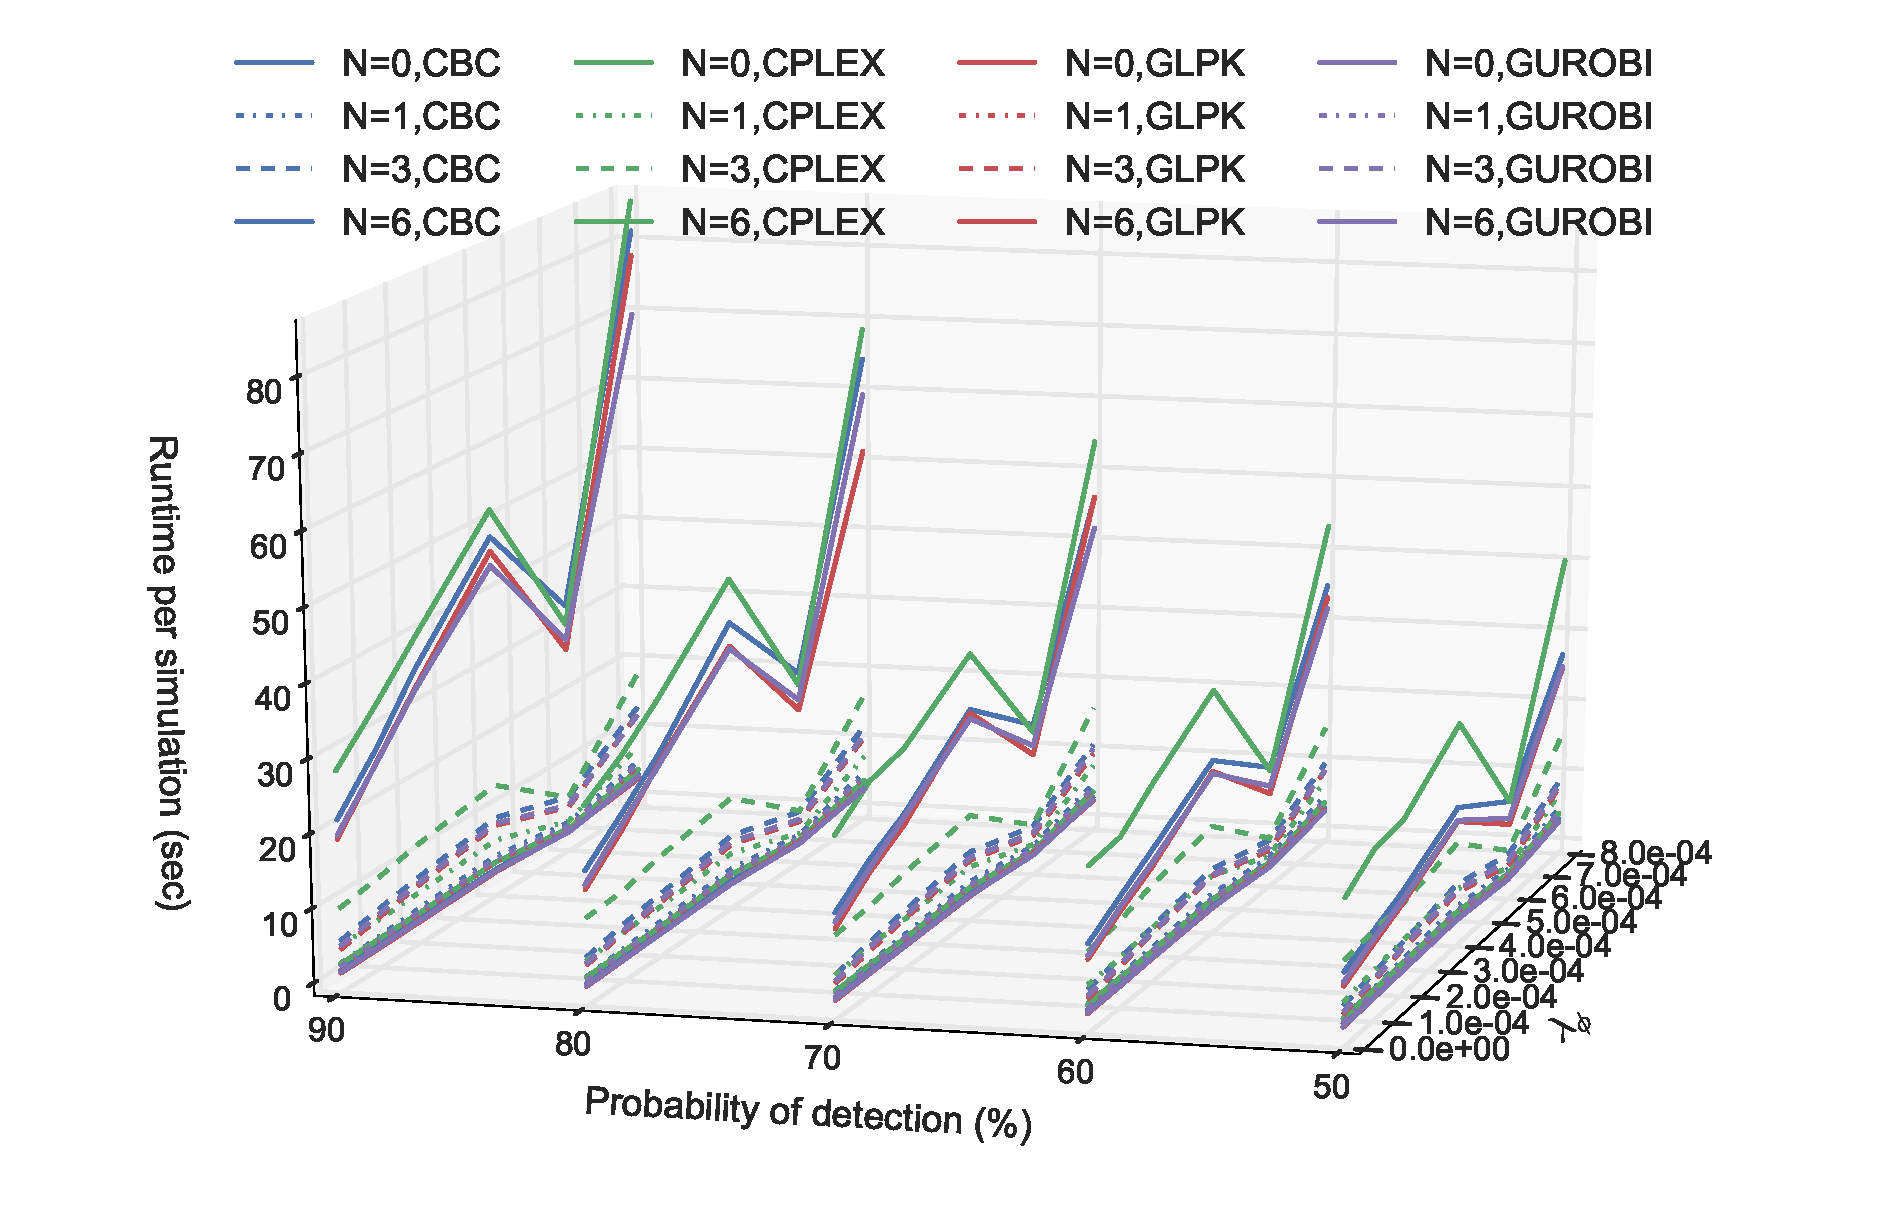
\includegraphics[clip, trim=0cm 1.5cm 0cm 0cm,width=\textwidth]{parallel_targets_1hz_runtime}
\caption{Runtime for scenario 5}
\label{fig:runtime_scenario_5}
\end{figure}

\begin{figure}[H]
\centering
\includegraphics[clip, trim=0cm 1.5cm 0cm 0cm,width=\textwidth]{{parallel_targets_0.5hz_runtime}.pdf}
\caption{Runtime for scenario 6}
\label{fig:runtime_scenario_6}
\end{figure}

\subsection{Track loss performance}
From the simulation results in Figure \ref{fig:dynamic_agents_full_cooperation_cropped} to \ref{fig:parallel_targets_1hz} in the appendix, it can be observed that the different solvers perform practically identically when it comes to track performance. From Figure \ref{fig:tracking_performance}, it can be seen that the number of lost tracks is proportional to the clutter level at an inverse proportional rate to the probability of detection $P_D$. An interesting observation is the return on investment regarding the number of scans to evaluate (N-scan). For instance, with $P_D=0.7$ the difference between $N=3$ and $N=6$ is marginal, at least when the clutter level is within reasonable levels ($\lambda_\phi < 4 \cdot 10^{-4}$). With $P_D=0.5$ is can be seen that the pay-off is much higher for the extra computational cost with 15\% improvement between $N=3$ and $N=6$.

Scenario 1-4 was simulated within a very small area where the targets had good separation both at the start and at the end of the simulation. This gives the algorithm more \glspl{scan} to figure out the correct association, after any multi-target conflicts that could arise when tracks are close to each other, and hence gives better track loss figures. In scenario 5-6 the targets start off spatially much closer and are moving faster. This leads to a situation more vulnerable to misdetections, and is an example of a situation where a high $N$-scan is beneficial.

\subsection{Time performance}
From Figure \ref{fig:runtime_scenario_1} to \ref{fig:runtime_scenario_6} it can be seen that the solvers have similar execution times, though with a very consistent difference in scenario 1 to 4. In these scenarios the \gls{glpk} solver is the fastest with 5-10 seconds compared with the slowest in these scenarios, \gls{cplex}. This trend is most likely caused by the different amount of overhead in the solvers, where IBM's \gls{cplex}, which is marked leading in many ways, might have way more initialization and setup procedures compared GNU's \gls{glpk}. In scenario 5 and 6, a different and more varying trend is visible. Here we see that both \gls{gurobi} and \gls{glpk} are fastest in different situations, and generally all other solvers than \gls{cplex} perform quite similar.

The run time increases linearly with the amount of clutter, which is expected as most of the operations run in the algorithm are based on tree operations with $O(E+V)$ run time. The structure in a track-tree implies that each vertex has one edge, hence any \gls{dfs} based operations will have run time  $O(2V)=O(V)$. The run time increases exponentially with the size of N, which is natural since the number of hypotheses that must be considered is exponentially larger.

\subsubsection{Bottle necks}
To study the effect parallel computation have on the tree growing task, a selected scan processing runtime was recorded with different amount of \gls{cpu} cores. Table \ref{tab:runtime_parallel} compares the run time averaged over 10 runs for the same scan, with different amount of parallel processes on a 4 core computer.

\begin{table}
\centering
\begin{tabular}{c c c c c c}
\bfseries Processes & \bfseries Total & \bfseries Grow & \bfseries Cluster & \bfseries Optimize & \bfseries Prune \\ \hline
\csvreader[head to column names]{{data/parallelTimeLog_ITK.csv}}{}
{\Processes & \Total & \Grow & \Cluster & \Optimize & \Prune \\\hline}
\end{tabular}
\caption{Runtime of a scan with different amount of processes (time in ms)}	
\label{tab:runtime_parallel}
\end{table}

Since the growing task is the only part of the algorithm that is utilizing on multiple cores, it is the only task that changes significantly. The multi processing of the growing task is implemented in a master-worker configuration, where the task is divided into $n-1$ equal chunks running on $n-1$ cores with the main process handling all the "worker" processes.  The run time increases when going from one to two processes, which is expected since the entire job is copied to another process, processed, and copied back. With any further increase in processor count, the execution time is expected to decline, which is also the case. At a certain core count, the time used to splitting up the task, distribute it to all the cores and collecting their results will become larger than the benefit of faster computation in each core. At this point, the overhead of parallizing the work leads to starvation of the workers and increased total run-time. On the four core machine, this limit is not reached, but by looking at Table \ref{tab:runtime_parallel_aws} in the appendix, displaying the runtime of the same program on a server with virtual \glspl{cpu}, it can be seen that the fastest execution time is with 6 cores. The scaling per core is worse on the virtualized server, possibly because the overhead of moving data to and forth the cores is larger. This means that running on a dedicated \gls{cpu} with more than four cores could yield higher optimal core count and thus better runtime performance. 


From Table \ref{tab:runtime_parallel_percentage}, we can see that the tree growing task is responsible for about one quarter of the run-time for this particular scan. Further analysis of the tree growing reveals that the creation of new nodes are the main contributor to the run time, with $97-98\%$ of the growing task.
\begin{table}
\centering
\begin{tabular}{c c c c c}
\bfseries Processes & \bfseries Grow & \bfseries Cluster & \bfseries Optimize & \bfseries Prune \\ \hline
\csvreader[head to column names,respect percent=true]{{data/parallelTimeLogPercentage_ITK.csv}}{}
{\Processes & \Grow \% & \Cluster \% & \Optimize \% & \Prune \% \\\hline }
\end{tabular}
\caption{Runtime distribution percentage}	
\label{tab:runtime_parallel_percentage}
\end{table}

\begin{table}
\centering
\begin{tabular}{c c c c c}
\bfseries Processes & \bfseries Search & \bfseries Predict & \bfseries Create & \bfseries Add \\ \hline
\csvreader[head to column names,respect percent=true]{{data/parallelTimeLogDistribution_ITK.csv}}{}
{\Processes & \Search \% & \Predict \% & \Create \% & \Add \% \\\hline }
\end{tabular}
\caption{Worker runtime distribution percentage}	
\label{tab:worker_parallel_percentage}
\end{table}
	%!TEX root = ../TTK4550-MHT.tex
\section{Discussion}
\label{sec:discussion}
The field of tracking and data association has been dominated by firstly military applications, and by secondly civil aviation control. Both of which are areas with hight performance demands and large development contracts \cite{Blackman2004}. Although much work is published on this topic, few comparisons have been made between actual implementations of different trackers and filters. This may to some extent be due to the nature of business secrets and military classifications to hide the intricate details that goes into an actual implementation and optimization of any tracking system. It is also, on a slightly more speculative note, due to disagreements about what kind of performance measures one should use. 

One of the main objectives for this work was to examine the feasibility of using off-the-shelf solvers to solve the assignment problem in a \gls{mht} system. This report have shown that all of the tested solvers ere capable of solving the assignment problem. It has also shown that there are some drawbacks with using off-the-shelf solvers. The largest ones beeing that the assignment problem must be written to a file that the solver can interpret. This is a major drawback with the chosen approach, but can be partially compensated for with fast \gls{ssd} in stead of traditional rotating hard drives. Another major drawback is the need for explicit enumeration of all hypotheses in the \gls{ilp} formulation, which is costly and in many situations unnecessary. This could possibly be addressed by column generating optimization methods \cite{Barnhart1998}, starting with a feasible set of columns and adding more and more columns (constraints) until it reaches the optimal assignment. Intuitively this makes sense, as most of the constraints will never be active, and therefore not needed for finding the optimal solution. This would, however, make the optimization a lot more tailor-made to this application, and render the usage of off-the-shelf solvers impossible.
	%!TEX root = ../TTK4550-MHT.tex
\section{Closing remarks}
\subsection{Conclusion}
This report has shown that off-the-shelf ILP solvers, both free and commercial, are capable solving the data association problem in a track oriented multiple hypothesis tracker. It has also shown that the tracking performance does benefit very little from more than $N=3$ scan history when the probability of detection $P_D > 70\%$, even with severe amounts of clutter.

\subsection{Future work}
One area where there might be substantial benefits is in more complex pruning and merging of hypotheses. By nature, many hypotheses will have very similar paths and could therefore be candidates for being merged to one. The danger with this is that the assignment problem could render infeasible and crash the algorithm. A novel approach could be to formulate the pruning as an optimization problem. With this approach it is possible to also remove hypotheses with a low score, subject to the problem still being feasible. 

I the maritime context, it could also be very beneficial to use the maritime AIS (Automatic Identification System) to aid the tracking. There are different approaches to include this extra set of data, with their pros and cons. One option could be to use the AIS track to weight the measurements from the radar, this way the measurement that are more likely to originate from a target is given a higher score. Another possibility is to do track-to-track fusion / filtering, where the best or N-best tracks from the radar are filtered with the tracks from the AIS system. A similar problem is tackled by Coraluppi in \cite{Coraluppi2000}.

Another improvement that would benefit the run time requirement is to parallelize  the algorithm. Since many of the operations in the algorithm are independent, they are excellent candidates for running in parallel. Today CPU's can be delivered with as many as 24 cores per die, and with hyper threading they can process op to 48 threads. With server grade motherboards capable of one to four CPU's, there is potential to run almost 200 threads if necessary. This would however be a pure brute force approach, which would push the boundary of how many targets the system would be able to track simultaneously, but not the run time as a function of the problem size.

A final but very important piece is also necessary for the system to  be complete, track initialization. As with AIS assisted tracking, there are plenty of ways to tackle this challenge. One alternative, and probably the most common for TOMHT is to run a separate system besides the tracking loop to initiate targets. This system can run i.e. recursive RANSAC, PDA-/JPDA-filter, with a selected criterion for birth. The most common is a N out of M threshold, where N and M is about 4 and 6. These separate initialization trackers can run on all measurements, or maybe preferably on the non-active measurements from the primary system. 
 \newpage
	
	\bibliographystyle{ieeetr}
	\bibliography{MHTbib}
\end{document}